\documentclass[12pt, letterpaper]{article}

% Font
\usepackage[utf8]{inputenc}
\usepackage{amsmath}
\usepackage{microtype}

% Format
\usepackage[letterpaper, margin = 1in]{geometry}
\setcounter{secnumdepth}{0}
\setlength{\parindent}{0.5in}
\usepackage[compact]{titlesec}  
\titleformat*{\section}{\centering\normalfont\normalsize\bfseries}
\titleformat*{\subsection}{\raggedright\normalfont\normalsize\bfseries}
\titleformat*{\subsubsection}{\raggedright\normalfont\normalsize\bfseries\itshape}
\usepackage{indentfirst}
\usepackage[hang,flushmargin]{footmisc}

% Header
\usepackage{fancyhdr}
\pagestyle{fancy}
\fancyhf{}
\setlength{\headheight}{14.5pt}
\renewcommand{\headrulewidth}{0pt}
\fancyhead[L]{`IRONIC' EFFECTS META-ANALYSIS}
\fancyhead[R]{\thepage}

% Links
\usepackage[colorlinks = true, linkcolor = black, urlcolor = black, citecolor = black]{hyperref} 

% Figures
\usepackage{graphicx}
\usepackage[labelfont = bf, font = small, labelsep = newline, singlelinecheck = false]{caption}

% Tables
\usepackage{booktabs}
\usepackage{tabularx}

% Line spacing
\usepackage[doublespacing]{setspace}

\begin{document}

\section{Abstract}

\noindent Growing evidence suggests that intergroup contact, psychology's
most-researched paradigm for reducing prejudice, has the `ironic' effect
of reducing support for social change in disadvantaged groups. We
conducted a preregistered meta-analytic test of this effect across 98
studies with 140 samples of 213,085 disadvantaged-group members. As
predicted, intergroup contact was, on average, associated with less
perceived injustice (\(r = -.07\)), collective action (\(r = -.06\)),
and support for reparative policies (\(r = -.07\)). However, these
associations were small, variable, and consistent with alternative
explanations. Moderator analyses found that associations were strongest
in studies of adults that measured intergroup contact directly and
examined short-term migration or post-colonial intergroup relations.
After controlling for the positive association of negative contact with
support for social change, positive contact was not associated with any
outcome in studies that measured both predictors. We close by
highlighting open questions about the relationship between intergroup
contact and social change.

\textit{Keywords:} intergroup contact, meta-analysis, perceived discrimination, collective
action, policy support

\newpage

\section{Meta-Analysis of the `Ironic' Effects of Intergroup Contact}

It is ironic that psychology's most-researched paradigm for reducing
prejudice---intergroup contact---should hinder, rather than help, social
change. Hundreds of studies have confirmed that intergroup contact is
associated with less negative feelings toward outgroup members (for a
meta-analysis, see Pettigrew \& Tropp, 2006). Most of these studies have
focused on advantaged-group members' contact experiences with
disadvantaged-group members (Tropp \& Pettigrew, 2005), guided by the
idea that reducing advantaged-group members' prejudice will prevent
interpersonal discrimination. Reducing prejudice, however, is rarely
enough to overcome institutional and structural discrimination. Instead,
as the 2020 Black Lives Matter protests have shown, social change often
requires political mobilization by the disadvantaged. Critics have
argued that, by fostering harmony and reducing conflict, intergroup
contact might distract disadvantaged-group members from the injustice
they face and, thereby, undermine their motivation for social change
(Dixon et al., 2005; Reicher, 2007; Wright, 2003). By reducing
disadvantaged-group members' opposition to injustice, intergroup contact
might thus have the `ironic' (Saguy et al., 2009), `sedative' (Çakal et
al., 2011), or `paradoxical' (Dixon et al., 2010) effect of hindering
social change.

Supporting this argument, initial studies provided evidence that contact
with advantaged-group members reduces disadvantaged-group members'
perceptions of injustice (Saguy et al., 2009), collective action (Çakal
et al., 2011), and support for reparative policies (Dixon et al., 2007).
Others, however, have pointed to conflicting evidence (Poore et al.,
2002) and argued that intergroup contact might instead make
discrimination more salient and, thereby, increase disadvantaged-group
members' support for social change (Pettigrew et al., 2011). In the
decade since the initial studies, many more studies have examined the
relationship between intergroup contact and support for social change in
disadvantaged groups. We present a systematic review and meta-analysis
of this growing literature to evaluate the evidence for and against the
`ironic' effects of intergroup contact.

\hypertarget{why-intergroup-contact-might-reduce-support-for-social-change}{%
\subsection{Why Intergroup Contact Might Reduce Support for Social
Change}\label{why-intergroup-contact-might-reduce-support-for-social-change}}

Researchers have put forward three hypotheses about how intergroup
contact might reduce support for social change in disadvantaged groups.

Perceived injustice---that is, perceiving unjust group-based deprivation
or discrimination against a disadvantaged ingroup---is a prerequisite to
instigating social change (van Zomeren et al., 2008). Researchers have
argued that positive contact with advantaged groups could contradict
perceptions of personal discrimination and, thereby, make group
discrimination appear less plausible (Dixon et al., 2010). Positive
contact could further reduce perceived injustice by emphasizing
commonalities over differences (Saguy et al., 2009) and by motivating
disadvantaged-group members to adopt system-justifying ideologies
(Sengupta \& Sibley, 2013). To the extent that it reduces perceived
injustice, intergroup contact reduces support for social change.

Collective action is any action directed at improving the conditions of
the disadvantaged ingroup (Wright et al., 1990). Collective action is
crucial to achieving social change because advantaged-group members
rarely give up their advantages without sustained pressure from
disadvantaged-group members (Blumer, 1958; for a review, see Dixon et
al., 2012). Researchers have argued that intergroup contact could
discourage disadvantaged-group members from engaging in collective
action by diminishing their perceived discrimination (Tropp et al.,
2012), by blurring boundaries between the disadvantaged ingroup and the
advantaged outgroup (Saguy et al., 2009), by reducing negative attitudes
toward the advantaged outgroup (Wright \& Lubensky, 2009), and by
quelling their anger (Hayward et al., 2018; Tausch et al., 2015). To the
extent that it discourages collective action, intergroup contact reduces
support for social change.

Reparative policies (e.g., affirmative action) can be effective means to
reduce social inequality. Disadvantaged-group members, who stand to
benefit from their implementation, are important advocates for these
policies. Researchers have argued that intergroup contact could diminish
disadvantaged-group members' support for redistributive policies by
creating sympathy for advantaged-group members (Dixon et al., 2007), by
fostering positive outgroup attitudes and reducing attention to
inequality (Saguy et al., 2009), and by increasing their endorsement of
system-justifying ideologies (Sengupta \& Sibley, 2013). To the extent
that it diminishes support for redistributive policies, intergroup
contact reduces support for social change.

To summarize, intergroup contact might hinder social change by reducing
disadvantaged-group members' perceived injustice, discouraging them from
engaging in collective action, and diminishing their support for
reparative policies.

\hypertarget{why-intergroup-contact-might-not-reduce-support-for-social-change}{%
\subsection{\texorpdfstring{Why Intergroup Contact Might \emph{not}
Reduce Support for Social
Change}{Why Intergroup Contact Might not Reduce Support for Social Change}}\label{why-intergroup-contact-might-not-reduce-support-for-social-change}}

Researchers have, however, argued that intergroup contact might
\emph{not} reduce support for social change and, in some circumstances,
might even \emph{increase} support for social change in disadvantaged
groups.

Some studies found evidence that intergroup contact is associated with
more, not less, support for social change in disadvantaged groups. Poore
et al. (2002) found that Inuit who had more exposure to non-indigenous
Canadians perceived greater discrimination against their group than
Inuit who lived in relative isolation. Similarly, researchers found
that, among members of various disadvantaged groups, intergroup contact
was associated with perceiving greater discrimination against the
disadvantaged ingroup (Dixon et al., 2017), perceiving status
differences between the advantaged outgroup and disadvantaged ingroup to
be less legitimate (Di Bernardo et al., 2019), and being more willing to
engage in collective action (Di Bernardo et al., 2019; Dixon et al.,
2017; Pereira et al., 2017). These findings align with the argument,
based in relative deprivation theory (Smith et al., 2012), that contact
with the advantaged provides an opportunity for the disadvantaged to
recognize their relative disadvantage and, thereby, can motivate the
disadvantaged to support social change (see Pettigrew et al., 2011;
Poore et al., 2002).

Other researchers have put forward alternative explanations for the
apparent `ironic' effects of intergroup contact. Whereas previous
studies had focused on positive contact experiences, recent studies
considered both positive and negative contact experiences as predictors
of support for social change. Researchers (Hayward et al., 2018; Reimer
et al., 2017) found negative contact with advantaged-group members to be
associated with greater perceived discrimination and stronger collective
action intentions, suggesting that negative contact experiences motivate
disadvantaged-group members to support social change. Reimer et al.
(2017) further found that, first, disadvantaged-group members who have
more positive contact also tend to have less negative contact and,
second, positive contact is not associated with perceived discrimination
or collective action after controlling for negative contact. Based on
these findings, Reimer et al. (2017) argued that the mobilizing effect
of negative contact could be an alternative explanation for the negative
relationship between positive contact and support for social change
observed in prior studies.

Another alternative explanation for the apparent `ironic' effects of
intergroup contact centers on intragroup contact. Whereas most studies
focused on contact with the advantaged outgroup, some studies examined
contact with the disadvantaged ingroup as a predictor of support for
social change. Sengupta et al. (2015) found ingroup contact to be
associated with decreased endorsement of system-justifying beliefs and
increased support for reparative policies benefiting the disadvantaged
ingroup, suggesting that contact with other ingroup members can motivate
disadvantaged-group members to support social change (see also Sengupta
\& Sibley, 2013). As outgroup contact places limits on how much ingroup
contact one can have (Pfister et al., 2020), disadvantaged-group members
who have more outgroup contact can be expected to have less ingroup
contact. Based on these observations, one might argue that the
mobilizing effect of ingroup contact could be an alternative explanation
for the negative association between outgroup contact and support for
social change observed in prior studies.

To summarize, intergroup contact might increase, not decrease, support
for social change in disadvantaged groups and the apparent `ironic'
effects might be based on spurious relationships between (positive)
intergroup contact and support for social change.

\hypertarget{purpose-of-the-present-study}{%
\subsection{Purpose of the Present
Study}\label{purpose-of-the-present-study}}

As societies are becoming more diverse, there are more opportunities for
members of different groups to come in contact with each other.
Psychologists disagree about what this means for disadvantaged-group
members' awareness of and opposition to social injustice. On the one
hand, researchers have argued that intergroup contact might reduce
disadvantaged-group members' perceived injustice, discourage them from
engaging in collective action, and diminish their support for reparative
policies. On the other hand, researchers have argued that intergroup
contact might not reduce, or even increase, support for social change in
disadvantaged groups. Settling this debate is important both because
intergroup contact is a promising means of reducing prejudice (Pettigrew
\& Tropp, 2006) and because political mobilization by the disadvantaged
is often crucial for achieving social change (see, for example,
Mazumder, 2018).

While narrative reviews of the growing literature on this topic have
been published (Hässler et al., 2021; MacInnis \& Hodson, 2019; McKeown
\& Dixon, 2017), we present the first systematic review and
meta-analysis of the relationship between intergroup contact and support
for social change in disadvantaged groups. To test the hypothesized
`ironic' effects of intergroup contact, we evaluate the evidence that
contact with advantaged-group members reduces disadvantaged-group
members' perceived injustice, discourages them from engaging in
collective action, and diminishes their support for reparative policies.

Our first objective was to systematically review the available evidence
and to evaluate its strengths and limitations. Our second objective was
to synthesize the available evidence to establish the direction and
magnitude of the relationships between intergroup contact and the three
outcomes. Doing so allowed us to determine whether the available
evidence supports a negative or positive (see Pettigrew et al., 2011)
relationship between contact and support for social change and to
estimate the strength of this relationship. Our third objective was to
estimate and explain the variability of this relationship across study
settings, designs, and other potential moderators. For example, we
examined whether any effects were confined to Western, Educated,
Industrialized, Rich, Democratic (WEIRD) countries, the cultural context
of most psychological research (Henrich et al., 2010). Our fourth
objective was to assess how robust the available evidence was to
publication bias. Our final objective was to explore the available
evidence for negative contact and ingroup contact as alternative
explanations of the apparent `ironic' effects of intergroup contact.

\hypertarget{method}{%
\section{Method}\label{method}}

\hypertarget{open-practices-statement}{%
\subsection{Open Practices Statement}\label{open-practices-statement}}

We prepared a protocol in accordance with the PRISMA-P statement (Moher
et al., 2015) and preregistered it on the Open Science
Framework.\footnote{\url{https://osf.io/ryuev/?view_only=8938ac6178914da98bdda1da4a6e27f0}}
Preregistration precludes undisclosed flexibility in study selection,
outcome selection, and other decisions that influence effect size
estimates---and thus prevents confirmation bias from determining the
conclusions of a meta-analysis (Lakens et al., 2016). We report
deviations from our protocol in the Supplemental Online Material (SOM).
We make data, analysis scripts, and the fully reproducible manuscript
available online.\footnote{\url{https://osf.io/w5tqv/?view_only=5cbf7ad5b2b449a7a0f4ada0337b802a}}

\hypertarget{eligibility-criteria}{%
\subsection{Eligibility Criteria}\label{eligibility-criteria}}

As preregistered, we considered all quantitative studies that included
participants of a relatively disadvantaged group (see \emph{Types of
Participants}), that manipulated or measured intergroup contact with a
relatively advantaged group (see \emph{Types of Predictor Variables}),
and that measured one or more of the following outcomes: perceptions or
expectations of injustice, collective action intentions and behaviours,
and/or support for policies that benefit or harm the participants'
ingroup (see \emph{Types of Outcome Variables}).

\hypertarget{types-of-participants}{%
\subsubsection{Types of Participants}\label{types-of-participants}}

We included studies with participants whose ingroup is disadvantaged (in
terms of status, power, or resources) relative to the outgroup they have
(or report to have) contact with.

\hypertarget{types-of-predictor-variables}{%
\subsubsection{Types of Predictor
Variables}\label{types-of-predictor-variables}}

We included studies if they measured or manipulated the quantity of,
quality of, and opportunity for contact with members of outgroups that
are relatively advantaged compared to the participants' ingroup. We
considered opportunity for contact, as it is a potential precursor to
and proxy for face-to-face contact, but not imagined or extended
contact. Similarly, we included studies that measured intergroup contact
indirectly by, for example, asking what proportion of someone's friends
were \emph{not} from the participants' ingroup.

\hypertarget{types-of-outcome-variables}{%
\subsubsection{Types of Outcome
Variables}\label{types-of-outcome-variables}}

\textbf{\emph{Perceived Injustice.}} We included studies that measured
perceptions that one is discriminated against because of one's group
membership, that one's group faces discrimination in society, that one's
group is relatively deprived compared to other groups, or that the
deprivation and/or discrimination faced by one's group is unjust and
illegitimate. We also considered expectations of fair treatment as the
reverse of perceived injustice. We included studies that measured
personal or group discrimination or both.

\textbf{\emph{Collective Action.}} We included studies that measured
observed, reported, or intended engagement in any action aimed at
improving the position of the participants' ingroup in society. This
included participating in protests, signing petitions, and any other
form of violent or nonviolent collective action.

\textbf{\emph{Policy Support.}} We included studies that measured
support for (or opposition to) policies and initiatives designed to
improve the position of the participants' ingroup in society, for
example, affirmative action policies.

\hypertarget{search-strategy}{%
\subsection{Search Strategy}\label{search-strategy}}

\begin{figure*}[t!]
\centering
\caption{Flow diagram illustrating the preregistered search strategy, study selection, and data collection}
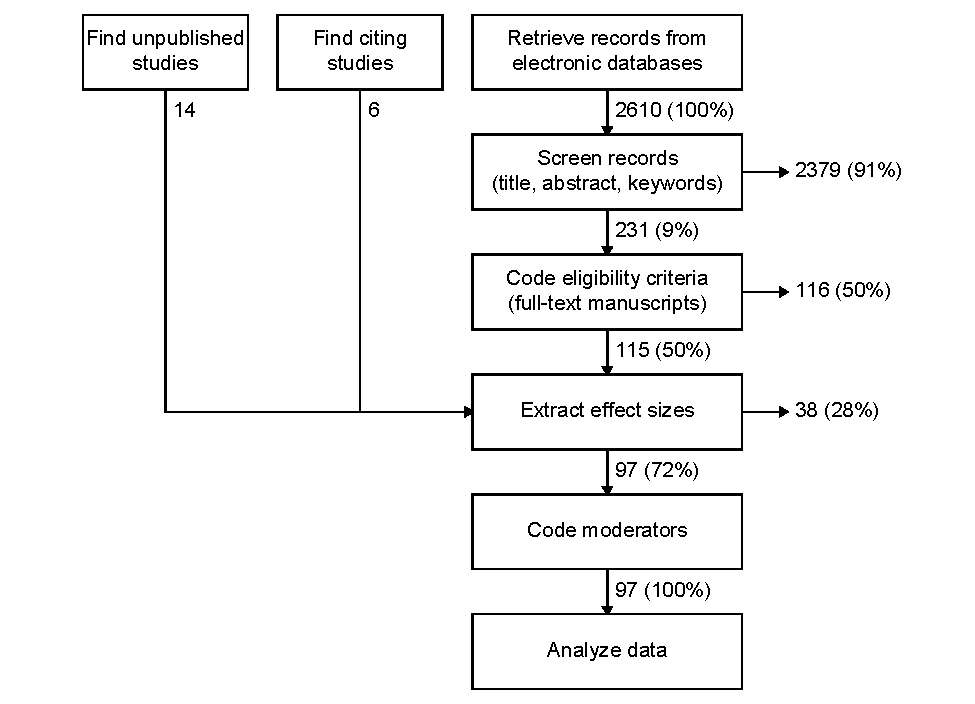
\includegraphics[scale=1]{../figures/figure-1}
\label{fig:f1}
\end{figure*}

As preregistered, we searched titles, abstract, and keywords for
relevant terms in four electronic databases. We searched for relevant
articles in the \emph{Scopus} and \emph{PsycINFO} databases. We searched
for gray literature in the \emph{ProQuest Dissertations and Theses}
database. We used similar non-exclusive search terms for all databases
(see SOM). We searched databases on April 1, 2019 and again on April 1,
2020. We exported records and relevant metadata from each database. We
removed duplicates using the \emph{revtools} package (Westgate, 2019).

To find unpublished studies, we sent a call to the mailing lists of
several professional organizations (see SOM). We also advertised on
social media and at relevant conferences. We directed researchers to an
online survey in which they answered questions about the eligibility of
their unpublished research and, if the research was eligible, provided
data on moderator variables and effect sizes. We also contacted experts
in the field, asking for unpublished research and other studies we might
have missed.

In addition, we used the \emph{Scopus} citation database to find records
that cited at least one of the published articles included in the
meta-analysis or at least one of three relevant review articles (Dixon
et al., 2012; Reicher, 2007; Wright \& Lubensky, 2009). This search
resulted in 2,075 records. Of these, we focused on 145 records that
cited at least three eligible studies or relevant reviews and looked for
eligible studies that were not among those from our original search.

\hypertarget{study-selection}{%
\subsection{Study Selection}\label{study-selection}}

As preregistered, we selected studies in three stages. First, we
screened records based on their title, abstract, and keywords. We
refined our coding strategy over three random samples of 100 records
until we achieved acceptable inter-rater agreement (\(\kappa_1 = .56\),
\(\kappa_2 = .60\), \(\kappa_3 = .79\)). We then divided the remaining
records between the two authors. For each record, one of the authors
coded whether the record met the eligibility criteria (yes, maybe, no),
or whether it was a relevant review article. We kept all records coded
as ``yes'' or ``maybe''. Second, both authors reviewed each of the
full-text manuscripts from the previous stage and coded whether any
study or sample in the manuscript fulfilled the preregistered
eligibility criteria (\(\kappa = .75\)). Third, we resolved any
disagreements (by consensus) and excluded ineligible records.

\hypertarget{data-collection}{%
\subsection{Data Collection}\label{data-collection}}

\hypertarget{effect-sizes}{%
\subsubsection{Effect Sizes}\label{effect-sizes}}

From all eligible records, we extracted correlation coefficients (\(r\))
as the relevant measure of effect size and extracted sample sizes
(\(n\)) to calculate standard errors for each sample's correlation
coefficients. When provided, we copied correlation coefficients from the
text or tables. When other effect-size measures were provided, we
converted them to correlation coefficients using common conversion
formulas (Borenstein et al., 2009). When effect sizes were not provided,
we attempted to contact the authors to obtain the relevant effect sizes.
We did not contact authors for studies that were more than twenty years
old as we considered it unlikely that authors still had access to the
underlying data. When we could not extract or obtain an effect size for
a study or sample, we either imputed missing correlation coefficients
from standardized beta coefficients (Peterson \& Brown, 2005) if
reported or excluded the study or sample if not.

\hypertarget{outcomes-selection}{%
\subsubsection{Outcomes Selection}\label{outcomes-selection}}

We collected effect sizes for all relationships between eligible
predictor and outcome variables. When more than one eligible measure was
reported, we extracted effect sizes for all of them. As preregistered,
we also extracted effect sizes for negative contact, ingroup contact,
group identification, and outgroup attitudes.

When a study reported effect sizes for more than one measure of
intergroup contact, we prioritized the predictor variable in the
preregistered analyses that measured the most intense or intimate form
of contact. As preregistered, we used the following ranking: cross-group
friendship \textgreater{} quality of contact/positive contact
\textgreater{} quantity of contact \textgreater{} opportunity for
contact. When it was unclear which of several predictor variables
measured the most intense form of contact, we combined and averaged
effect sizes.

When a study reported effect sizes for more than one measure of one of
the three outcome variables, we selected effect sizes for the
preregistered analyses as follows: For perceived injustice, we
prioritized the measure closest to perceptions of injustice against the
participants' ingroup (rather than against the participants themselves);
when it was ambiguous which measure that was, we combined and averaged
effect sizes across outcome measures. For collective action, we
prioritized the measure that was the primary focus of the reported
analyses; otherwise, we combined and averaged effects sizes across
outcome measures. For policy support, we combined and averaged effect
sizes for all policies designed to improve the position of the
participants' ingroup in society.

Some study designs resulted in more than one effect size for the same
measure: When a longitudinal study reported results from more than two
waves, we prioritized effect sizes spanning the inter-survey interval
closest to one year. If a longitudinal study reported results from more
than two waves and spanned multiple years, we combined and averaged
effect sizes from each one-year inter-survey interval. In the
preregistered analyses, we included the cross-lagged partial correlation
between the relevant predictor variable (at time 1) and outcome variable
(at time 2) controlling for initial levels of the outcome variable (at
time 1). When an experimental or quasi-experimental study reported
comparisons between more than two conditions, we prioritized the effect
size that compared two conditions that most closely resembled generic
contact and no-contact conditions.

\begin{figure*}
\centering
\caption{Overview of the relevant literature}
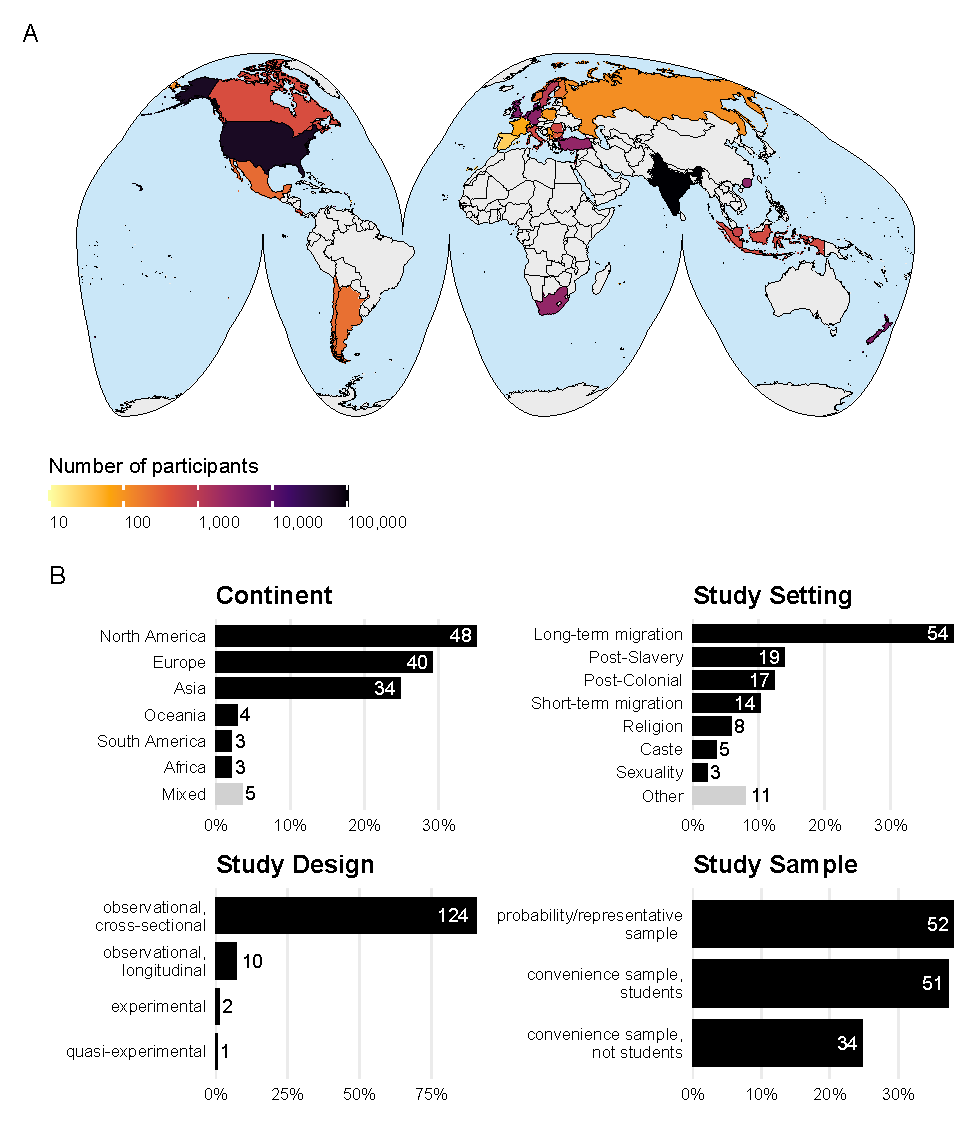
\includegraphics[scale=1]{../figures/figure-2}
\caption*{\textit{Note.} \textbf{A} Map of all countries included in the meta-analysis with combined sample sizes. \textbf{B} Proportion of eligible samples in each category as well as the absolute number of samples in each category.}
\label{fig:f2}
\end{figure*}

\hypertarget{potential-moderators}{%
\subsubsection{Potential Moderators}\label{potential-moderators}}

In addition to extracting and selecting effect sizes for the
preregistered analyses, we collected data on a broad range of potential
moderators. All moderators that required subjective assessments were
coded by both authors. We calculated inter-rater agreement (Cohen's
\(\kappa\)) and resolved all disagreements by consensus.

\textbf{\emph{Study Setting.}} For each sample, we recorded in what
country (or countries) the data was collected (\(\kappa = .97\)) and
what the disadvantaged ingroup and the advantaged outgroup were. We
categorized each sample's setting according to whether the source of the
groups' relative inequality was long-term migration (e.g., Asian
Americans), short-term migration (e.g., international students), slavery
(e.g., Black Americans), colonization (e.g., Māori, Black South
Africans), religion, caste, sexuality, or another distinction
(\(\kappa = .85\)).

\textbf{\emph{Study Design.}} We categorized each study as either
observational and cross-sectional, observational and longitudinal,
quasi-experimental, experimental, an intervention, or other
(\(\kappa = .85\)). We categorized each sample as either a student
convenience sample, a non-student convenience sample, a probability or
representative sample, or another kind of sample (\(\kappa = .73\)). We
categorized the age group(s) in each sample as children (\(\leq 12\)
years), adolescents (13--18 years), or adults (\(\geq 18\) years;
\(\kappa = .64\)).

\textbf{\emph{Study Intention.}} We coded whether or not each study was
conducted with the intention to examine the effects of intergroup
contact on one or more of the three outcome measures (\(\kappa = .48\)).
We did not achieve acceptable inter-rater agreement in our initial
coding. After refining our coding criteria, we re-coded all studies by
consensus.

\textbf{\emph{Publication status.}} For each study, we coded whether it
was published, unpublished, or an unpublished dissertation based on the
information source from which we obtained it.

\textbf{\emph{Predictor Variables.}} For each measure of intergroup
contact, we coded whether it assessed contact with the specific
advantaged outgroup of interest directly---or whether it assessed
contact indirectly by, for example, asking what proportion of someone's
friends were not from the participants' ingroup or what proportion of
residents in someone's neighbourhood were from the relevant outgroup
(\(\kappa = .82\)).

\textbf{\emph{Outcome Variables.}} For each measure of perceived
injustice, we coded whether it refered to specific instances of
discrimination, to a more general perception of discrimination, or to
both (\(\kappa = .67\)) and whether it assessed personal discrimination,
group discrimination, or both (\(\kappa = .84\)).

\textbf{\emph{Cultural Distance.}} We also used the index developed by
Muthukrishna et al. (2020), where available, to quantify each country's
cultural distance from the United States, which represents the cultural
context of most psychological research (Henrich et al., 2010).

\hypertarget{analysis-strategy}{%
\subsection{Analysis Strategy}\label{analysis-strategy}}

\hypertarget{preregistered-analyses}{%
\subsubsection{Preregistered Analyses}\label{preregistered-analyses}}

We transformed correlation coefficients to Fisher's \(z\) which is
unbounded and has a normal sampling distribution: \begin{align*} 
z & = \frac{1}{2} \ln\left(\frac{1 + r}{1 - r}\right) \\ \sigma & = \frac{1}{\sqrt{n - 3}} \end{align*}
where \(r\) is the sample correlation coefficient, \(z\) is the
transformed effect size, \(n\) is the sample size, and \(\sigma\) is the
standard error of the transformed effect size.

We estimated effect sizes using Bayesian random-effects meta-analysis
models in \emph{RStan} (Stan Development Team, 2020) which modeled the
\emph{z}-transformed correlation coefficients with a normal likelihood
function:
\begin{align*} z_{ij} &\sim \text{Normal}(\theta_{ij}, \sigma_{ij}) \\ \theta_{ij} &= \begin{cases} \mu + \beta_j\tau_J & \text{if } I_j = 1 \\ \mu + \beta_j\tau_J + \beta_i\tau_I & \text{if } I_j > 1 \end{cases} \\ \end{align*}
where \(z_{ij}\) is the observed effect size in sample \(i\) of study
\(j\), \(\sigma_{ij}\) is the sample standard error, and \(\theta_{ij}\)
is the estimated effect size. We estimated \(z_{ij}\) as a function of
the mean effect size \(\mu\) and of two varying (random) intercepts,
\(\beta_i\) and \(\beta_j\), with the corresponding standard deviations,
\(\tau_I\) and \(\tau_J\). We used the non-centered parameterization to
model the random effects. For studies that contained only one sample
(\(I_j = 1\)), we only included \(\beta_j\tau_J\), the study-wise
deviation from the mean effect size \(\mu\). For studies that contained
more than one sample (\(I_j > 1\)), we also estimated \(\beta_i\tau_I\),
the sample-wise deviation from the study-specific effect size.

Models assigned weakly informative prior distributions to all
parameters. The prior distribution for the mean effect size,
\(\mu \sim \text{Normal}(0, 0.31605)\), was centered around 0 and
concentrated 50\% of the most plausible values between \(r = -.21\) and
\(r = .21\). We focus on \(|r| = .21\) because it corresponds to the
mean effect size observed in both Pettigrew and Tropp's (2006)
meta-analysis of the contact literature and Richard et al.'s (2003)
meta-analysis of effect sizes across a century of social-psychological
research. The prior distribution for the standard deviation of random
effects, \(\tau \sim \text{Half-Cauchy}(0, 0.3)\), allocated 30\% of
plausible values below \(\tau = 0.15\) and had a wide tail. We focus on
\(\tau = 0.15\) because it corresponds to the standard deviations
observed in both Pettigrew and Tropp's (2006) and Richard et al.'s
(2003) meta-analyses. We chose this prior distribution in line with
recommendations by Williams et al.~(2018).

Bayesian inference involves choosing a likelihood function and prior
distributions. A likelihood function links the observed data to one or
more model parameters and states how likely the observed data are given
different values of said model parameters. Prior distributions state how
plausible different values of said model parameters are before
considering the observed data. Bayesian inference applies Bayes' theorem
to update prior distributions in light of the observed data to produce
posterior distributions. In contrast to \emph{p}-values and confidence
intervals, the resulting posterior distributions have a straightforward
interpretation as stating how plausible different values of the model
parameters are given the observed data. We report point estimates, based
on the median of posterior samples, and uncertainty intervals, based on
the quantiles of posterior samples, that enclose the 95\% most plausible
estimates. In addition, we report the posterior probability, based on
the proportion of posterior samples below zero, that the mean effect
size is negative.

\hypertarget{other-analyses}{%
\subsubsection{Other Analyses}\label{other-analyses}}

We also conducted non-preregistered analyses to estimate to what extent
moderator variables explained heterogeneity in the estimated effect
sizes, to what extent meta-biases influenced the estimated effect sizes,
and to what extent the three outcome variables were associated with two
alternative predictor variables, ingroup contact and negative contact.

\hypertarget{results}{%
\section{Results}\label{results}}

\hypertarget{search-results}{%
\subsection{Search Results}\label{search-results}}

Figure 1 shows a flow diagram illustrating our search strategy, study
selection, and data collection. Our preregistered search strategy
returned 2,610 unique records from electronic databases. Of these, we
excluded 2,379 (91\%) ineligible records after screening titles,
abstracts, and keywords. Of the remaining 231 records, we excluded 116
(50\%) ineligible records after reviewing full-text manuscripts. We
supplemented these records with 15 unpublished studies and 6 records
that cited at least three relevant works. Of 136 eligible studies, we
had to exclude 38 (28\%) studies for which we could not extract or
impute any relevant effect size. At each stage, we also excluded studies
that used the same data as another study. Our final sample comprised
effect sizes from \(J = 98\) studies spanning \(N = 213,085\)
participants in \(I = 140\) samples (for a complete list of studies, see
SOM).

Figure 2 provides a qualitative overview of the literature. Even though
most participants came from studies conducted in India (\(N = 104,639\))
and the United States (\(N = 60,983\); Figure 2a), most samples were
collected in North America (\(I = 48\)) and Europe (\(I = 43\)), with
few samples from South America and Africa (Figure 2b). Most samples
focused on relative inequalities that resulted from long-term migration
(\(I = 59\)), slavery (\(I = 19\)), colonization (\(I = 19\)), and
short-term migration (\(I = 14\)). With few exceptions, studies used
observational, cross-sectional survey designs. Samples sizes ranged from
64 to 49,764 (\(\textit{Mdn} = 287\)). Unlike most psychological
research, 2 in 5 samples used probability or representative sampling. Of
all samples, 55\% (\(I = 77\)) were collected with the intention to
examine the effects of intergroup contact on the outcomes considered in
this meta-analysis. Many studies instead examined acculturation
processes (Berry, 1997) and measured intergroup contact and perceived
injustice without hypothesizing that the former would influence the
latter. Together, these observations highlight both limitations and
strengths of the empirical literature.

\hypertarget{preregistered-analyses-1}{%
\subsection{Preregistered Analyses}\label{preregistered-analyses-1}}

As preregistered, we ran three random-effects meta-analysis models, one
for each outcome variable. Figure 3 shows posterior distributions from
these analyses.

\begin{figure*}[t!]
\centering
\caption{Posterior distributions from the preregistered random-effects meta-analysis models}
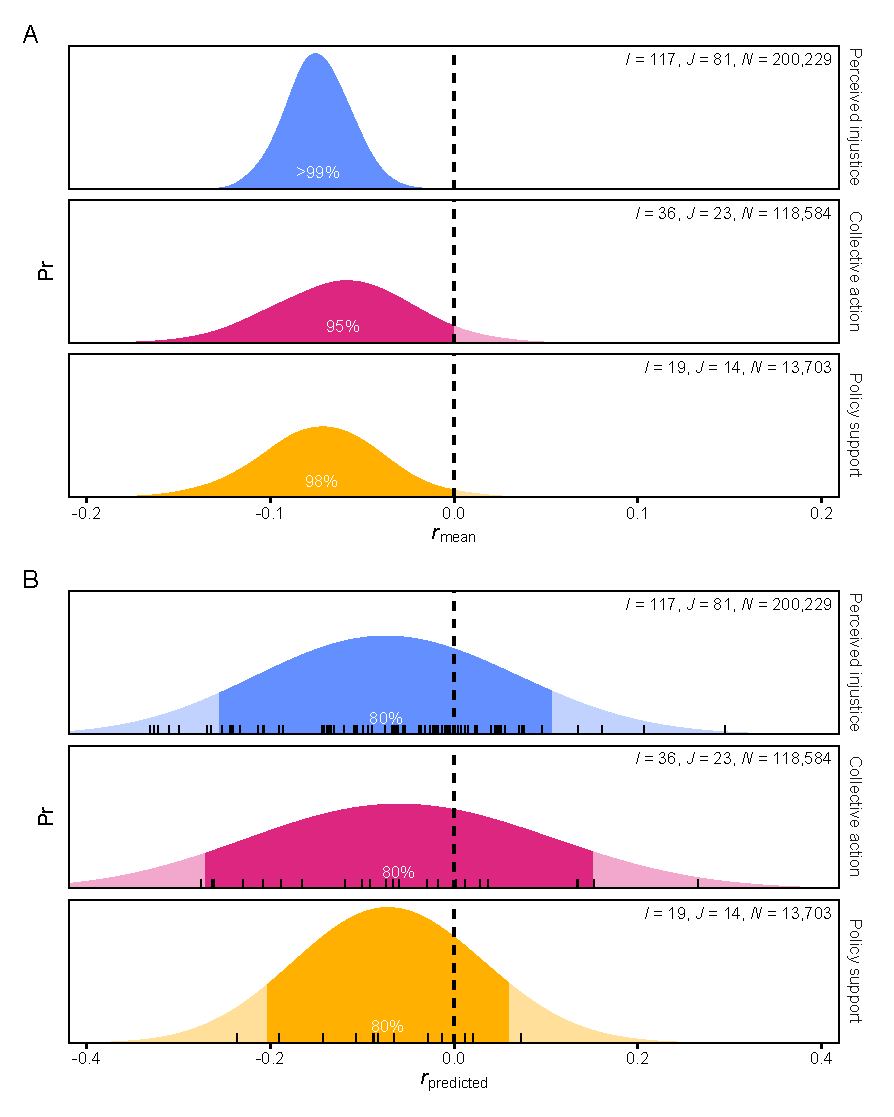
\includegraphics[scale=1]{../figures/figure-3}
\caption*{\textit{Note.} \textbf{A} Posterior distributions for the mean correlation coefficients, highlighting the proportion of posterior samples for which $r_\text{mean} < 0$. \textbf{B} Posterior predictive distributions of study-wise correlation coefficients, highlighting the 80\% most common effect sizes, with point estimates for the correlation coefficients for all studies in the sample.}
\label{fig:f3}
\end{figure*}

\textbf{\emph{Perceived Injustice.}} Across 203,637 participants from
126 samples in 86 studies, we found strong evidence for a weak negative
association (\(r = -.07, [-.10, -.04]\)) between intergroup contact and
perceived injustice, with \(>99.9\%\) of posterior samples for the mean
correlation coefficient falling below zero. We found evidence that
correlation coefficients varied across studies
(\(\tau_J = .14, [.11, .17]\)) and across samples within studies
(\(\tau_I = .08, [.05, .12]\)). Based on these analyses, we predicted
that 80\% of studies would result in correlation coefficients between
-.25 and .11 and that 31\% of studies would find a \emph{positive}
correlation between intergroup contact and perceived injustice. Our
analyses suggested that researchers would need sample sizes of at least
2,542 participants to find significant associations (\(\alpha = .05\),
two-sided) in 80\% of their studies.\footnote{Sample sizes are based on
  posterior predictions which implied that, for 80\% of studies, the
  absolute correlation coefficient would be \(|r| > .039\) for perceived
  injustice, \(|r| > .045\) for collective action, and \(|r| > .035\)
  for policy support.}

\textbf{\emph{Collective Action.}} Across 119,085 participants from 37
samples in 24 studies, we found some evidence for a weak negative
association (\(r = -.06, [-.13, .02]\)) between intergroup contact and
collective action, with \(93.6\%\) of posterior samples for the mean
correlation coefficient falling below zero. We found evidence that
correlation coefficients varied across studies
(\(\tau_J = .16, [.12, .23]\)) and across samples within studies
(\(\tau_I = .09, [.06, .14]\)). Based on these analyses, we predicted
that 80\% of studies would result in correlation coefficients between
-.27 and .16 and that 36\% of studies would find a \emph{positive}
correlation between intergroup contact and collective action. Our
analyses suggested that researchers would need sample sizes of at least
1,882 participants to find significant associations (\(\alpha = .05\),
two-sided) in 80\% of their studies.

\textbf{\emph{Policy Support.}} Across 13,703 participants from 19
samples in 14 studies, we found evidence for a weak negative association
(\(r = -.07, [-.14, -.00]\)) between intergroup contact and policy
support, with \(98.1\%\) of posterior samples for the mean correlation
coefficient falling below zero. We found evidence that correlation
coefficients varied across studies (\(\tau_J = .10, [.06, .18]\)) and,
to a lesser extent, across samples within studies
(\(\tau_I = .03, [.00, .12]\)). Based on these analyses, we predicted
that 80\% of studies would result in correlation coefficients between
-.21 and .07 and that 25\% of studies would find a \emph{positive}
correlation between intergroup contact and policy support. Our analyses
suggested that researchers would need sample sizes of at least 3,208
participants to find significant associations (\(\alpha = .05\),
two-sided) in 80\% of their studies.

As preregistered, we ran another three random-effects meta-analysis
models to estimate the relationships between the three outcome
variables. As we were not interested in the direction of these
relationships, we used cross-sectional correlation coefficients as
effect sizes for longitudinal studies. Across 111,753 participants from
25 samples in 14 studies, we found evidence for a moderate association
(\(r = .31, [.23, .38]\)) between perceived injustice and collective
action. Across 6,244 participants from 12 samples in 9 studies, we found
evidence for a moderate association (\(r = .23, [.08, .35]\)) between
perceived injustice and policy support. Across 8,558 participants from 6
samples in 3 studies, we found evidence for a moderate association
(\(r = .30, [.14, .42]\)) between collective action and policy support.

\hypertarget{robustness-checks}{%
\subsubsection{Robustness Checks}\label{robustness-checks}}

As preregistered, we conducted two kinds of robustness checks. First, we
assessed to what extent our findings were sensitive to choosing
narrower, \(\mu \sim \text{Normal}(0, 0.1)\), or wider,
\(\mu \sim \text{Normal}(0, 1)\), prior distributions. Choosing narrower
or wider prior distribution did not affect mean effect size estimates
for perceived injustice (\(\Delta r = -.00, [-.05, .04]\) and
\(\Delta r = .00, [-.05, .05]\)), collective action
(\(\Delta r = -.01, [-.11, .09]\) and \(\Delta r = .00, [-.11, .10]\)),
and policy support (\(\Delta r = -.01, [-.10, .08]\) and
\(\Delta r = .00, [-.09, .10]\)). Second, we assessed to what extent our
findings were sensitive to including or excluding influential studies by
repeating the preregistered analyses \(J\) times while leaving out one
of \(J\) studies each time and by calculating the mean absolute
difference (\emph{MAD}) for the estimated mean effect size across
left-out studies. For perceived injustice
(\(\textit{MAD} = .02, [.01, .04]\)), collective action
(\(\textit{MAD} = .04, [.02, .09]\)), and policy support
(\(\textit{MAD} = .03, [.02, .08]\)), the \emph{MAD} was small. Leaving
out the most influential study, for example, did not change estimates of
the mean effect size for the three outcomes
(\(\Delta r = -.00, [-.05, .04]\); \(\Delta r = .02, [-.08, .12]\);
\(\Delta r = -.02, [-.11, .07]\)). These analyses showed that our
findings were robust to choosing different prior distributions and to
excluding influential studies.

\hypertarget{moderator-analyses}{%
\subsection{Moderator Analyses}\label{moderator-analyses}}

We conducted three kinds of moderator analyses. As we had insufficient
numbers of effect sizes to examine moderators for collective action and
policy support, we report results for these outcomes in the SOM.

\begin{figure*}
\centering
\caption{Estimated effect sizes for the association between intergroup contact and perceived injustice as a function of various categorical moderator variables}
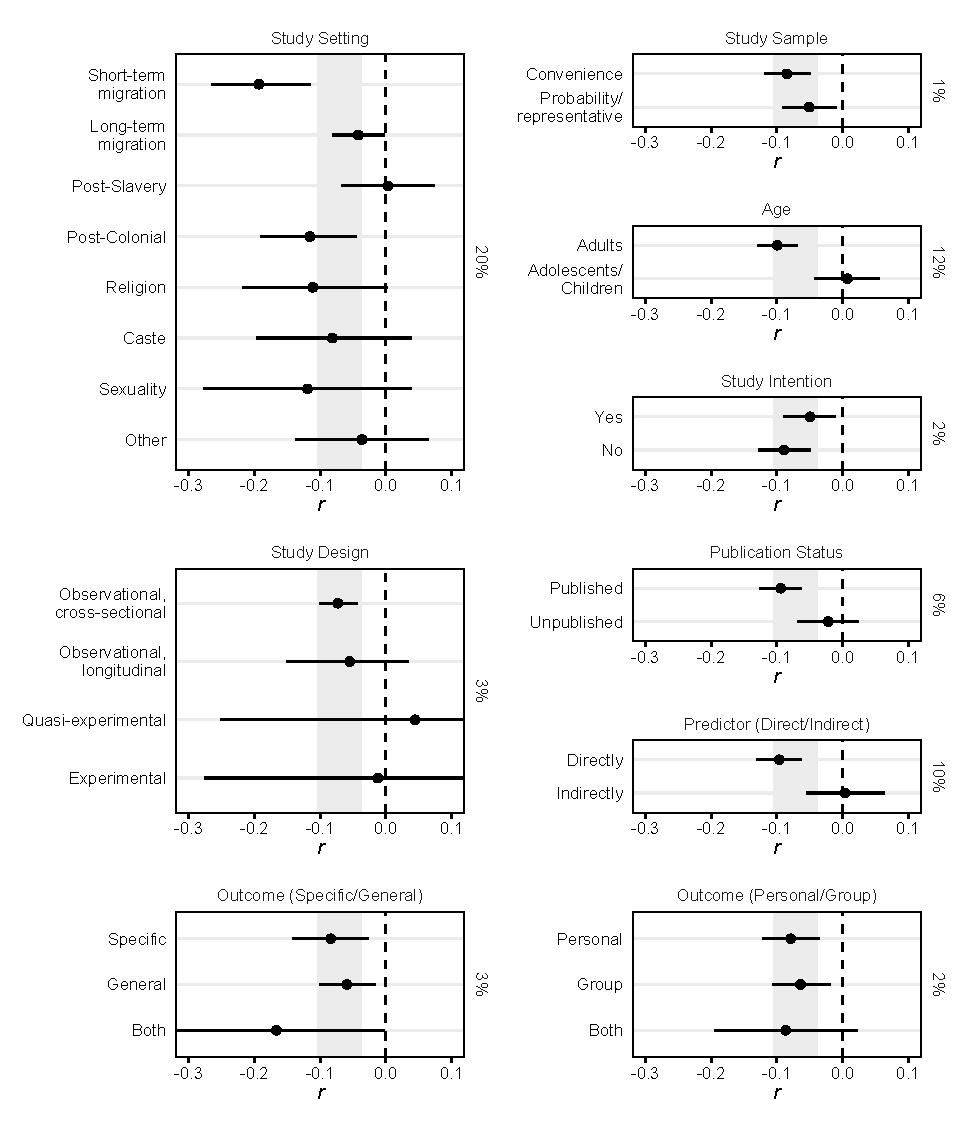
\includegraphics[scale=1]{../figures/figure-4}
\caption*{\textit{Note.} Intervals enclose the 95\% most plausible estimates of the category-specific effect size. Shaded ribbons enclose the 95\% most plausible estimates of the mean effect size from the main analyses. Percentages indicate the estimated between-sample variance explained by each moderator variable.}
\label{fig:f4}
\end{figure*}


\begin{figure*}
\centering
\caption{Estimated effect size as a function of cultural distance from the United States, with point estimates and uncertainty intervals for each country}
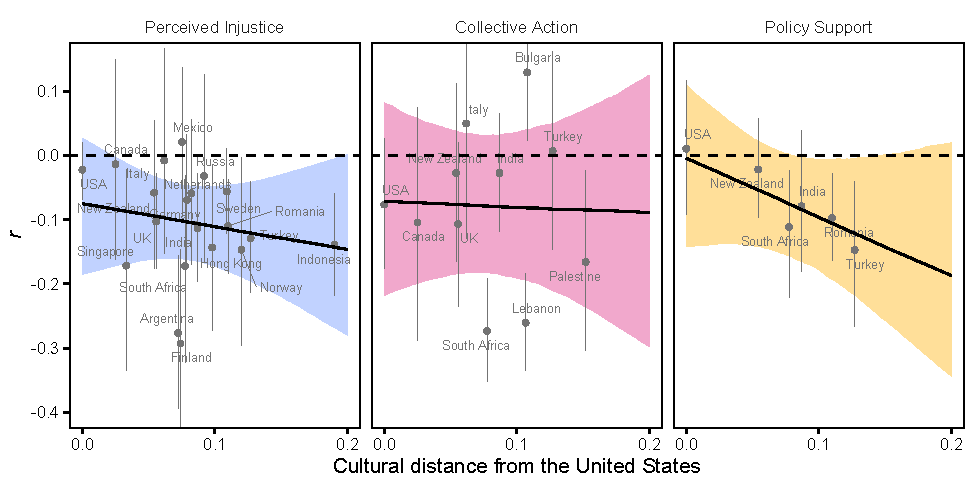
\includegraphics[scale=1]{../figures/figure-5}
\caption*{\textit{Note.} We had data from too few countries to reach firm conclusions about the direction of these associations for perceived injustice ($\beta = -0.38, [-1.45, 0.72]$; $\Pr (\beta < 0) = 75.7\%$), collective action ($\beta = -0.09, [-1.60, 1.37]$; $\Pr (\beta < 0) = 55.1\%$), and policy support ($\beta = -0.92, [-2.13, 0.55]$; $\Pr (\beta < 0) = 90.3\%$).}
\label{fig:f5}
\end{figure*}

\begin{figure*}
\centering
\caption{Results from the random-effects meta-regression tree analysis}
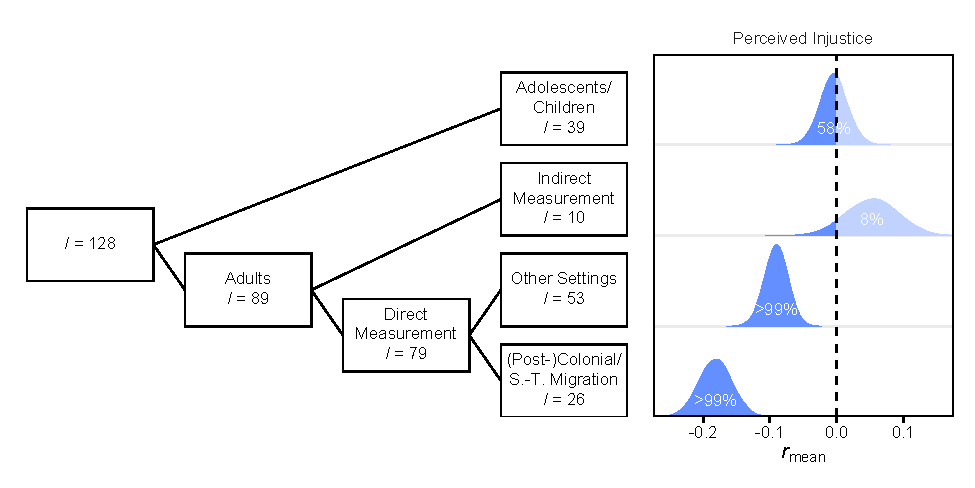
\includegraphics[scale=1]{../figures/figure-6}
\caption*{\textit{Note.} Posterior distributions for the estimated correlation coefficient in each leaf of the meta-regression tree, highlighting the proportion of posterior samples for which $r_\text{mean} < 0$.  S.-T. Migration = Short-Term Migration.}
\label{fig:f6}
\end{figure*}

First, we used meta-regression models to examine categorical moderator
variables which we expected to explain heterogeneity in effect sizes
across samples. As Figure 4 shows, we found that the setting of the
study (\(R^2 = 20\%\)), participants' age group (\(R^2 = 11\%\)), and
whether intergroup contact was measured directly or indirectly
(\(R^2 = 10\%\)) explained the most variance across effect sizes.

Second, we used meta-regression models to estimate effect sizes as a
function of each country's cultural distance from the United States
(Muthukrishna et al., 2020). Because cultural distance is a
country-level moderator variable, we estimated random intercepts to
account for both country-specific deviations from the mean effect size
and sample-specific deviations from the country-specific effect size. As
Figure 5 shows, we found that cultural distance from the United States
tended to be associated with larger effect sizes---although we had data
from too few countries to reach any firm conclusions.

Third, we used meta-regression trees to discover interactions between
moderator variables that best explained heterogeneity in effect sizes
(Li et al., 2017, 2020). Figure 6 shows the resulting meta-regression
model, which explained more variance across samples than any individual
moderator (\(R^2 = 31\%\)). We found that intergroup contact was
associated with less perceived injustice only in studies that focused on
adults and that measured intergroup contact directly. Among these
studies, this association was stronger in settings in which the groups'
relative inequality stemmed from short-term migration or colonization
(\(r = -.18, [-.23, -.13]\)) than in other settings
(\(r = -.09, [-.13, -.06]\)).

\hypertarget{meta-bias}{%
\subsection{Meta Bias}\label{meta-bias}}

\begin{figure*}
\centering
\caption{Unadjusted ($\bullet$) and adjusted ($\circ$) point estimates with confidence intervals from the random-effects meta-analysis (RMA), the PET-PEESE estimator, the three-parameter selection model (3PSM), the \textit{p}-uniform* estimator, and the subgroup analysis}
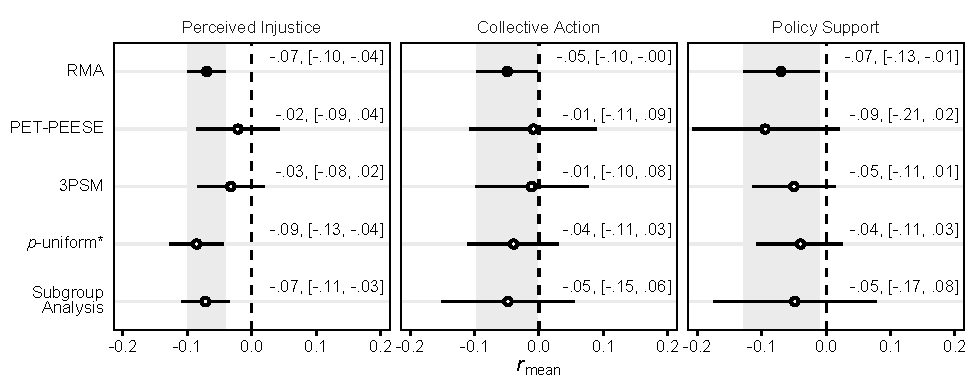
\includegraphics[scale=1]{../figures/figure-7}
\label{fig:f7}
\end{figure*}

Developing methods to detect and correct for publication bias and other
meta-biases is an active area of research, with no single method
outperforming all others (Carter et al., 2019). Following Carter et
al.'s recommendations, we compared results of several methods to adjust
meta-analytic estimates for publication bias: the PET-PEESE estimator
(Stanley \& Doucouliagos, 2014); the three-parameter selection model
(3PSM; Vevea \& Hedges, 1995); and the \emph{p}-uniform* estimator (van
Aert \& Assen, 2018). In addition, we ran a subgroup analysis that
included only studies that were not published or not conducted with the
intention to examine the effects of intergroup contact on any of the
outcomes---and that, therefore, can be assumed to have not been affected
by publication bias. As these methods do not use Bayesian statistics, we
compared adjusted estimates to unadjusted estimates from a
random-effects meta-analysis estimated with restricted maximum
likelihood estimation using the \emph{metafor} package (Viechtbauer,
2010).

Figure 7 shows adjusted and unadjusted estimates with confidence
intervals for the three outcomes. Comparing adjusted and unadjusted
estimates shows that the PET-PEESE and 3PSM methods tended to estimate
the mean correlation coefficients to be closer to zero than the
unadjusted estimate, with all confidence intervals including zero. The
\emph{p}-uniform* method and the subgroup analysis tended to estimate
the mean correlations coefficients to be closer to the unadjusted
estimates, with the confidence interval for perceived injustice---but
not for the other outcomes---excluding zero. All methods, however,
resulted in confidence intervals that largely overlapped with, but were
wider than, the confidence intervals around the unadjusted estimates.
This reflects the reduced power of the various methods to correct for
meta-biases when sample sizes are small, effect sizes are heterogeneous,
or publication bias is strong (Carter et al., 2019). Therefore, we did
not find evidence for publication bias---but also did not find
conclusive evidence against it.

\hypertarget{alternative-predictors}{%
\subsection{Alternative Predictors}\label{alternative-predictors}}

\begin{figure*}[t!]
\centering
\caption{Posterior distributions from the random-effects meta-analysis models with alternative predictor variables}
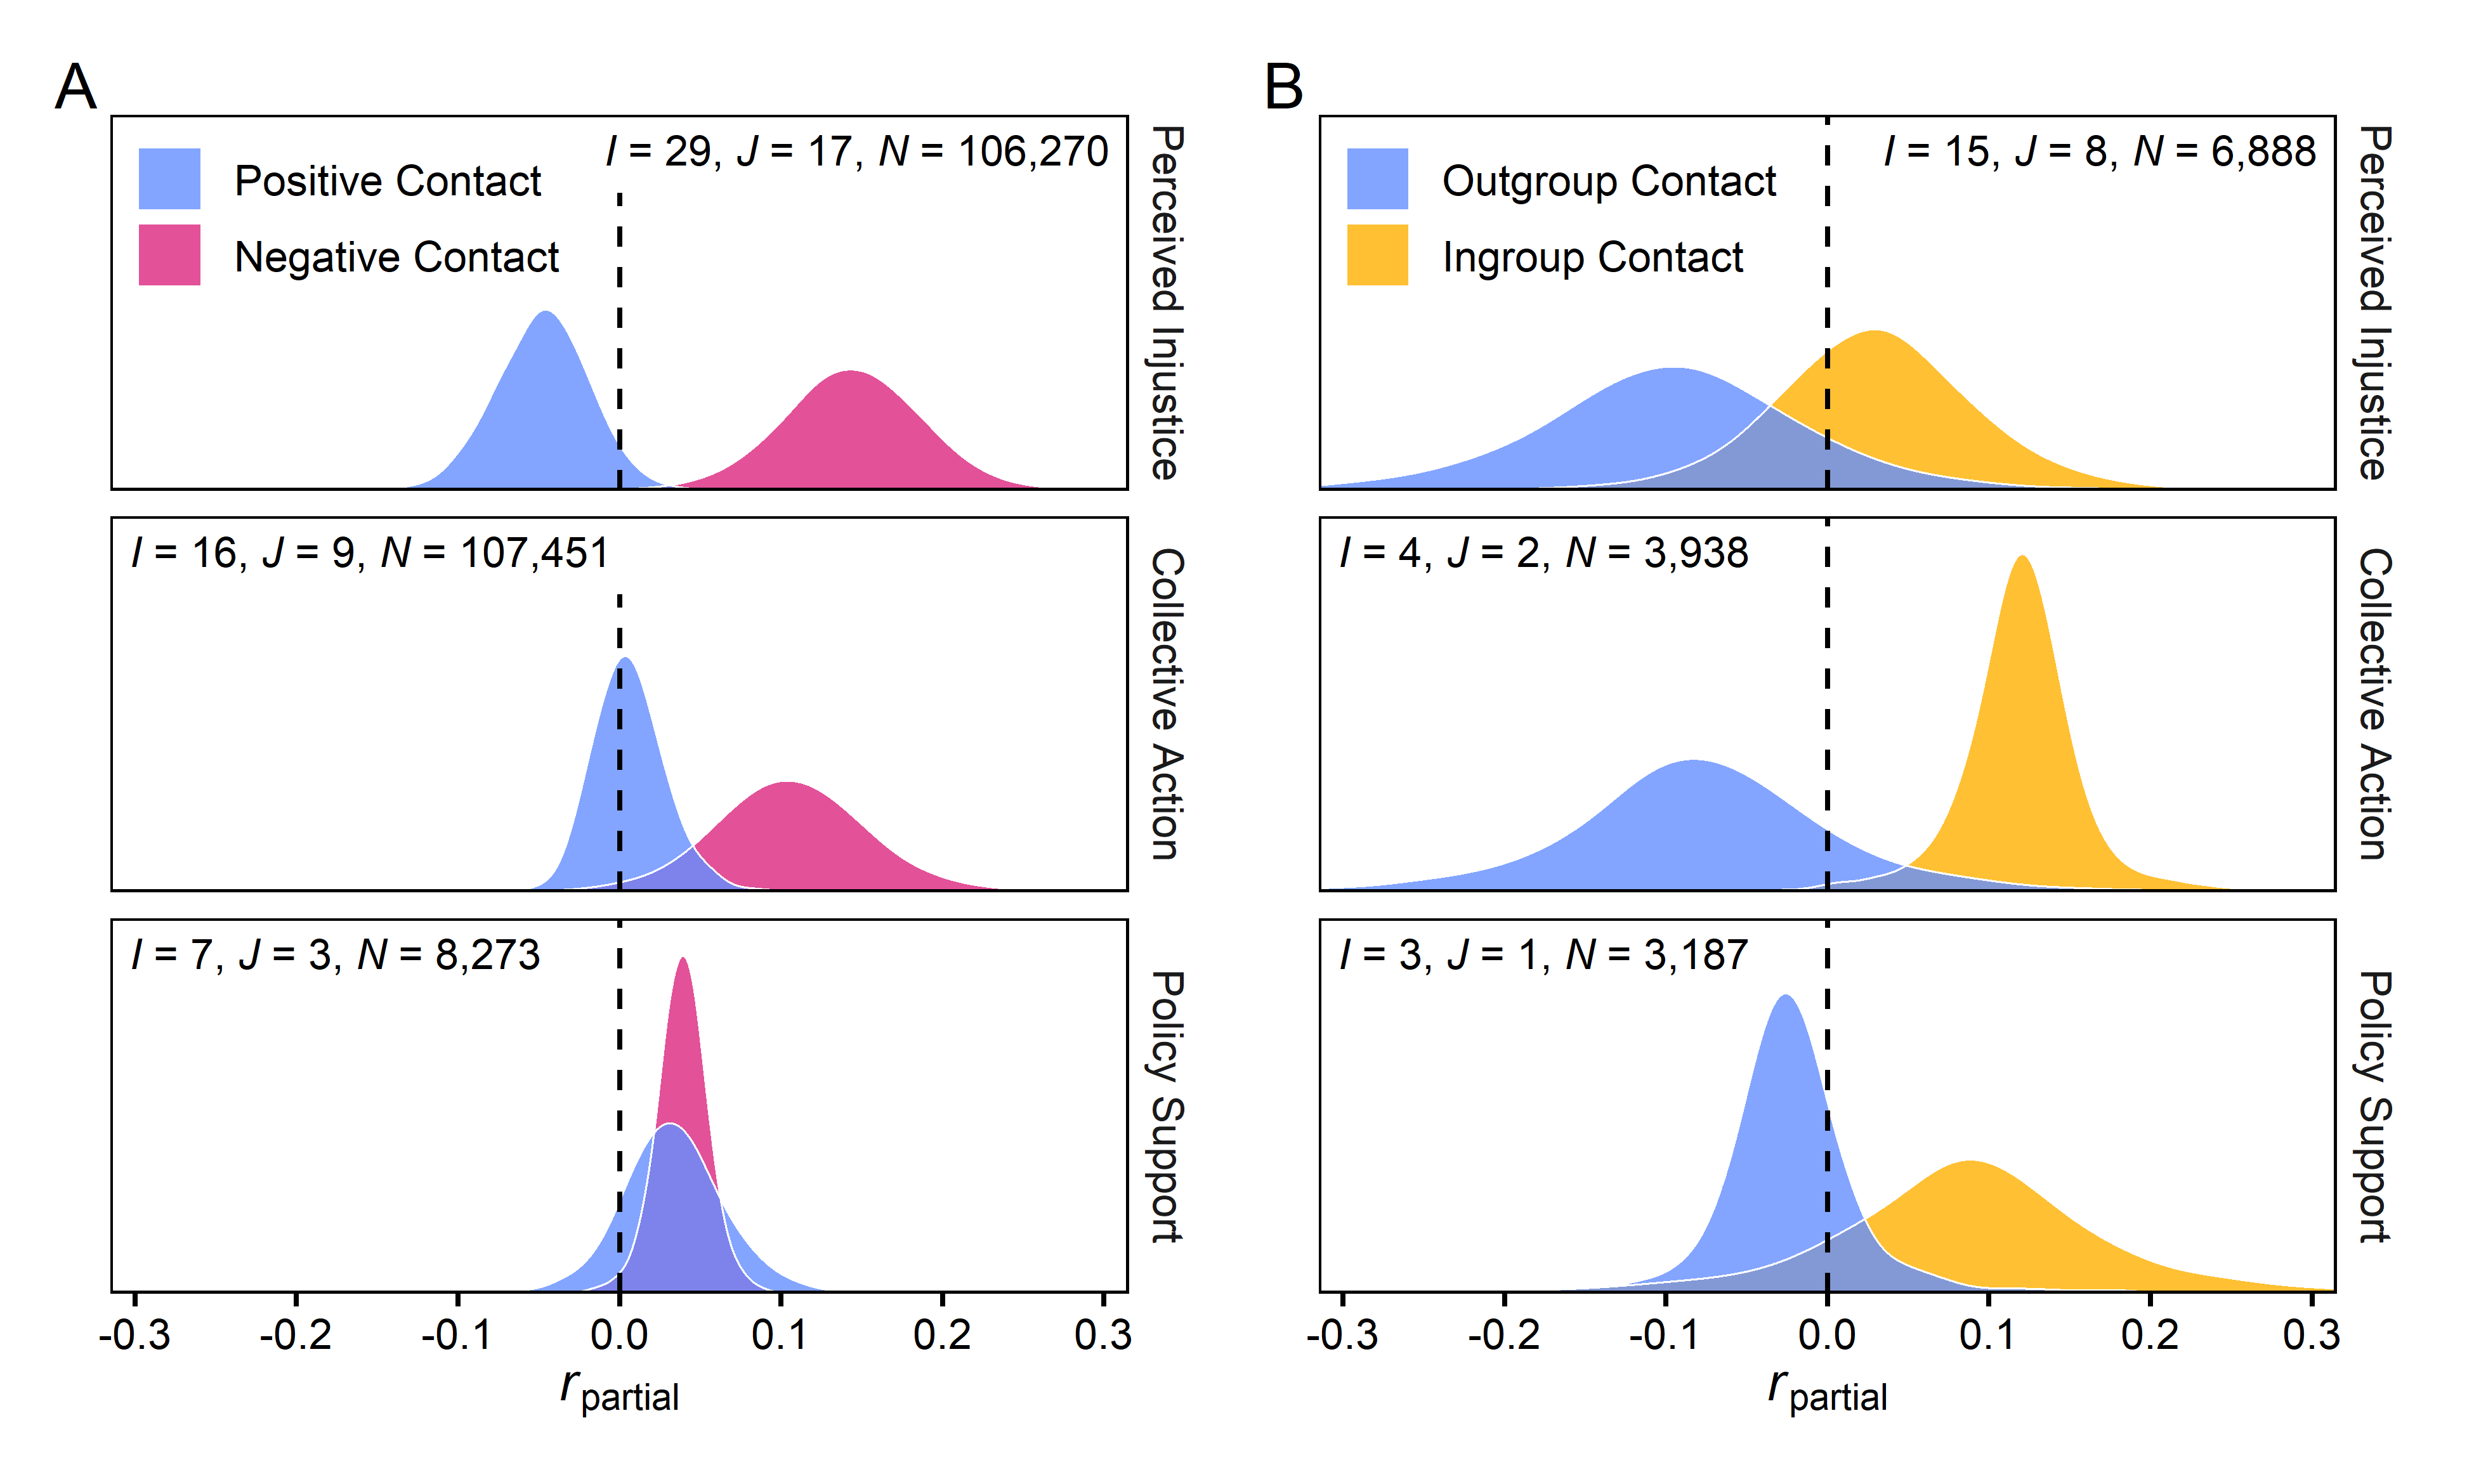
\includegraphics[scale=1]{../figures/figure-8}
\label{fig:f8}
\end{figure*}

We ran three random-effects meta-analysis models estimating the partial
correlations of positive and negative contact with each outcome, using
effect sizes from all studies that measured both predictors (Figure 8a).
By using partial correlations, we estimated the effect of one form of
contact while controlling for the other. Across 106,270 participants
from 29 samples in 17 studies, we found somewhat stronger evidence for a
positive association between negative contact and perceived injustice
(\(r = .14, [.06, .23]\); \(\Pr (r > 0) = 99.9\%\)) than for a negative
association between positive contact and perceived injustice
(\(r = -.05, [-.10, .01]\); \(\Pr (r < 0) = 95.6\%\)). Across 107,451
participants from 16 samples in 9 studies, we again found stronger
evidence for a positive association between negative contact and
collective action (\(r = .11, [.01, .20]\); \(\Pr (r > 0) = 98.4\%\))
than for a negative association between positive contact and collective
action (\(r = .00, [-.03, .06]\); \(\Pr (r < 0) = 40.7\%\)). Across
8,273 participants from 7 samples in 3 studies, we also found stronger
evidence for a positive association between negative contact and policy
support (\(r = .04, [.00, .07]\); \(\Pr (r > 0) = 98.3\%\)) than for a
negative association between positive contact and policy support
(\(r = .03, [-.03, .10]\); \(\Pr (r < 0) = 12.7\%\)). Across 111,153
participants from 31 samples in 18 studies, we found a negative
association between positive and negative contact
(\(r = -.16, [-.25, -.07]\); \(\Pr (r < 0) = 99.8\%\)).

We ran three random-effects meta-analysis models that estimated the
partial correlations of ingroup and outgroup contact with each outcomes,
using effect sizes from all studies that measured both predictors
(Figure 8b). Across 6,888 participants from 15 samples in 8 studies, we
found insufficient evidence for associations of ingroup contact
(\(r = .03, [-.10, .15]\); \(\Pr (r > 0) = 69.0\%\)) and outgroup
contact (\(r = -.10, [-.26, .07]\); \(\Pr (r < 0) = 89.2\%\)) with
perceived injustice. Across 3,938 participants from 4 samples in 2
studies, we found stronger evidence for a positive association between
ingroup contact and collective action (\(r = .12, [.03, .20]\);
\(\Pr (r > 0) = 99.1\%\)) than for a negative association between
outgroup contact and collective action (\(r = -.08, [-.25, .10]\);
\(\Pr (r < 0) = 85.5\%\)). Across 3,187 participants from 3 samples in 1
study, we found insufficient evidence for associations of ingroup
contact (\(r = .09, [-.13, .27]\); \(\Pr (r > 0) = 86.2\%\)) and
outgroup contact (\(r = -.03, [-.12, .08]\); \(\Pr (r < 0) = 78.5\%\))
with policy support. Across 6,888 participants from 15 samples in 8
studies, we found a positive association between ingroup and outgroup
contact (\(r = .25, [.10, .34]\); \(\Pr (r > 0) = 99.7\%\)).

\hypertarget{discussion}{%
\section{Discussion}\label{discussion}}

There is an emerging consensus that intergroup contact has the `ironic'
effect of undermining support for social change in disadvantaged groups.
We conducted a preregistered meta-analytic test of this effect across 96
studies with 137 samples of 211,360 disadvantaged-group members. We
found that, based on the available evidence, the associations of
intergroup contact with perceived injustice (\(\Pr (r < 0) > 99.9\%\)),
collective action (\(\Pr (r < 0) = 93.6\%\)), and support for reparative
policies (\(\Pr (r < 0) = 98.1\%\)) were, on average, much more likely
to be negative than positive. Thus, our meta-analysis seems to support
the emerging consensus. However, our findings qualify this conclusion in
several important ways.

First, the estimated effect sizes for the average associations of
intergroup contact with perceived injustice (\(r = -.07\)), collective
action (\(r = -.06\)), and policy support (\(r = -.07\)) were small.
Across the three outcomes, the 95\% most plausible estimates included
effect sizes between \(r = -.14\) and \(r = .02\). Effect sizes were
thus much smaller than for the association between contact and prejudice
in minority (\(r = -.18\)) and majority (\(r = -.23\)) groups (Tropp \&
Pettigrew, 2005).\footnote{Comparing standardized effect sizes assumes
  that the two outcomes are of equal importance. That is not always the
  case: for example, a drug that reduces mild symptoms by 0.20 standard
  deviations is not better than a drug that reduces deaths by 0.10
  standard deviations.} Small effects can still be important if they
accumulate over time or across people. For example, even a small change
in policy attitudes could, if it affects enough people, sway a tight
election. Cumulative effects, however, should not be assumed without an
empirical or theoretical rationale (Funder \& Ozer, 2019).

Second, the estimated effect sizes varied across studies. For example,
we estimated that 31\% of studies find a positive association between
intergroup contact and perceived injustice. While the between-study
heterogeneity is comparable to that in other meta-analyses (e.g.,
Pettigrew \& Tropp, 2006), it supports Pettigrew et al.'s (2011)
argument that, at least in some circumstances, intergroup contact
renders discrimination \emph{more} salient.

A combination of moderators explained about a third of the between-study
variance in the association between intergroup contact and perceived
injustice. We found that, on average, this association was negative only
in studies of adults that measured contact \emph{directly} (e.g., by
asking about the number of friends from the advantaged outgroup). This
suggests that, as hypothesized, the `ironic' effects result from direct
contact and not from other contextual factors. We also found that, on
average, effect sizes were greater for studies in (post-)colonial
settings or on short-term migration than for studies in other contexts.
Future research should systematically investigate variance in how
contact affects support for social change across settings and cultures.

Third, the available evidence is almost entirely from cross-sectional,
observational studies and thus consistent with alternative explanations
for the observed associations. Support for social change could reduce
intergroup contact rather than the other way around. For example,
disadvantaged-group members involved in collective action might avoid
forming friendships with advantaged-group members. Alternatively, the
observed associations could be spurious with both being caused by an
unobserved confounder. For example, a disadvantaged-group member's
socioeconomic status might both expose them to more advantaged-group
members and reduce their perception of injustice. Future research should
prioritize longitudinal studies to confirm the direction of the observed
associations and (field) experiments to rule out confounding and other
alternative explanations.\footnote{Published research includes only
  three longitudinal studies (Koschate et al., 2012; Reimer et al.,
  2017; Tropp et al., 2012), all of which conflated within-person change
  and between-person stability (Hamaker et al., 2015), two experimental
  studies with a no-contact control condition (Becker et al., 2013;
  Droogendyk et al., 2016), and two intervention studies (Reimer et al.,
  2021; Shani \& Boehnke, 2017).}

Fourth, the observed association between intergroup contact and support
for social change could be confounded by an alternative predictor that
\emph{increases} support for social change. Supporting Reimer et al.'s
(2017) argument, we found that positive intergroup contact was not
associated with support for social change after controlling for negative
contact which, in turn, was associated with \emph{greater} support for
social change. We found mixed evidence for ingroup contact as an
alternative explanation for the `ironic' effects of intergroup contact
(Sengupta et al., 2015) but note that few studies measured both ingroup
and outgroup contact. Going forward, researchers should clarify which
aspects of intergroup contact should theoretically affect support for
social change---and include measures that allow testing both the
hypothesized and competing explanations.

Finally, we cannot rule out that biases in the literature caused our
meta-analysis to overestimate the `ironic' effects of intergroup
contact. Publication bias could have prevented studies that found
positive or non-significant associations from entering the published
literature. We used various methods to detect and correct for
publication bias, yet did not find conclusive evidence for or against
publication bias. That said, 61\% of samples were either not collected
with the intention to study the effects of intergroup contact on a
relevant outcome (45\%) or from unpublished studies (32\%)---and thus
unlikely to have been affected by publication bias. Another bias that
could have affected our findings is that researchers made data-dependent
decisions when analyzing data that inflate false-positive findings
(Gelman \& Loken, 2014). Future research should use preregistration and
other methods to prevent undisclosed flexibility in data collection and
analysis.\footnote{Only one preregistered study has been published
  (Hässler et al., 2020).}

To conclude, our preregistered meta-analysis found some evidence that
intergroup contact reduces perceived injustice, discourages collective
action, and diminishes support for reparative policies in disadvantaged
groups---but also showed that the estimated effect sizes were small,
variable, and consistent with alternative explanations. Our research was
motivated by the broader question whether intergroup contact helps or
hinders social change. By examining the narrower question whether
intergroup contact diminishes support for social change in disadvantaged
groups, we tested the most prominent hypothesis explaining how
intergroup contact might \emph{hinder} social change. We did not
consider whether intergroup contact might \emph{help} social change by
reducing prejudice (for a critical perspective, see Dixon et al., 2012)
or by motivating advantaged-group members to acknowledge and challenge
social inequality (Tropp \& Barlow, 2018). Still, we hope that our
meta-analytic review motivates researchers to address the open questions
about how intergroup contact relates to support for social change in
disadvantaged groups.

\hypertarget{references}{%
\section{References}\label{references}}

\noindent References marked with an asterisk are studies included in the
meta-analysis.

\begingroup

\noindent \setlength{\parindent}{-0.5in} \setlength{\leftskip}{0.5in}
\small

\hypertarget{refs}{}
\leavevmode\hypertarget{ref-3201}{}%
*Albzour, M., Penic, S., Nasser, R., \& Green, E. G. T. (2019). Support
for ``normalization'' of relations between Palestinians and Israelis,
and how it relates to contact and resistance in the West Bank.
\emph{Journal of Social and Political Psychology}, \emph{7}(2),
978--996. \url{https://doi.org/10.5964/jspp.v7i2.877}

\leavevmode\hypertarget{ref-2023}{}%
*Bagci, S. C. (2014). \emph{Cross-ethnic friendships in multiethnic
educational settings: Consequences for psychological, academic and
motivational outcomes among young adolescents} {[}Doctoral dissertation,
Goldsmiths, University of London{]}.
\url{https://doi.org/10.25602/GOLD.00011030}

\leavevmode\hypertarget{ref-2395}{}%
*Bagci, S. C., \& Stathi, S. (2020). \emph{Secure and insecure ingroup
identification as mediators between identity threat and psychological
well-being and intergroup bias} {[}Manuscript in preparation{]}. Faculty
of Arts and Social Sciences, Sabanci University.

\leavevmode\hypertarget{ref-423}{}%
*Bagci, S. C., Stathi, S., \& Piyale, Z. E. (2019). Imagined contact
facilitates acculturation, sometimes: Contradicting evidence from two
sociocultural contexts. \emph{Cultural Diversity and Ethnic Minority
Psychology}, \emph{25}(4), 539--552.
\url{https://doi.org/10.1037/cdp0000256}

\leavevmode\hypertarget{ref-322}{}%
*Bagci, S. C., \& Turnuklu, A. (2019). Intended, unintended, and unknown
consequences of contact: The role of positive-negative contact on
outgroup attitudes, collective action tendencies, and psychological
well-being. \emph{Social Psychology}, \emph{50}(1), 7--23.
\url{https://doi.org/10.1027/1864-9335/a000355}

\leavevmode\hypertarget{ref-414}{}%
*Bagci, S. C., Turnuklu, A., \& Bekmezci, E. (2018a). Cross-group
friendships and psychological well-being: A dual pathway through social
integration and empowerment. \emph{British Journal of Social
Psychology}, \emph{57}(4), 773--792.
\url{https://doi.org/10.1111/bjso.12267}

\leavevmode\hypertarget{ref-2257}{}%
*Bagci, S. C., Turnuklu, A., \& Bekmezci, E. (2018b). The buffering role
of in-group identification and intergroup contact on the association
between perceived discrimination and mental health. \emph{Journal of
Community \& Applied Social Psychology}, \emph{28}(5), 293--305.
\url{https://doi.org/10.1002/casp.2357}

\leavevmode\hypertarget{ref-2396}{}%
*Bagci, S. C., Verkuyten, M., Koc, Y., Turnuklu, A., Piyale, Z. E., \&
Bekmezci, E. (2020). Being tolerated and being discriminated against:
Links to psychological well-being through threatened social identity
needs. \emph{European Journal of Social Psychology}, \emph{50}(7),
1463--1477. \url{https://doi.org/10.1002/ejsp.2699}

\leavevmode\hypertarget{ref-2075}{}%
*Becker, J. C., Wright, S. C., Lubensky, M. E., \& Zhou, S. (2013).
Friend or ally: Whether cross-group contact undermines collective action
depends on what advantaged group members say (or don't say).
\emph{Personality and Social Psychology Bulletin}, \emph{39}(4),
442--455. \url{https://doi.org/10.1177/0146167213477155}

\leavevmode\hypertarget{ref-1045}{}%
*Benner, A. D., \& Wang, Y. (2017). Racial/ethnic discrimination and
adolescents' well-being: The role of cross-ethnic friendships and
friends' experiences of discrimination. \emph{Child Development},
\emph{88}(2), 493--504. \url{https://doi.org/10.1111/cdev.12606}

\leavevmode\hypertarget{ref-berry_immigration_1997}{}%
Berry, J. W. (1997). Immigration, acculturation, and adaptation.
\emph{Applied Psychology}, \emph{46}(1), 5--34.
\url{https://doi.org/10.1111/j.1464-0597.1997.tb01087.x}

\leavevmode\hypertarget{ref-blumer_race_1958}{}%
Blumer, H. (1958). Race prejudice as a sense of group position.
\emph{The Pacific Sociological Review}, \emph{1}(1), 3--7.
\url{https://doi.org/10.2307/1388607}

\leavevmode\hypertarget{ref-2397}{}%
*Bond, J., \& Dixon, J. (2020). \emph{White and Black UK residents'
support for collective action for the removal of public symbols
associated with historical racism in England} {[}Unpublished dataset{]}.
The Open University.

\leavevmode\hypertarget{ref-borenstein_introduction_2009}{}%
Borenstein, M., Hedges, L. V., Higgins, J. P. T., \& Rothstein, H. R.
(2009). \emph{Introduction to meta-analysis}. Wiley.

\leavevmode\hypertarget{ref-2398}{}%
*Bracegirdle, C. (2020). \emph{Social network study of two diverse
schools in Northern England} {[}Unpublished dataset{]}. University of
Oxford.

\leavevmode\hypertarget{ref-carter_correcting_2019}{}%
Carter, E. C., Schönbrodt, F. D., Gervais, W. M., \& Hilgard, J. (2019).
Correcting for bias in psychology: A comparison of meta-analytic
methods. \emph{Advances in Methods and Practices in Psychological
Science}, \emph{2}(2), 115--144.
\url{https://doi.org/10.1177/2515245919847196}

\leavevmode\hypertarget{ref-480}{}%
*Castro, V. S. (2005). Discriminación percibida y autoestima en jóvenes
de grupos minoritarios y mayoritarios en Costa Rica {[}Perceived
discrimination and self-esteem among ethnic majority and minority youths
in Costa Rica{]}. \emph{Revista Interamericana de Psicología},
\emph{39}(1), 93--106.

\leavevmode\hypertarget{ref-1914}{}%
*Castro Solano, A., \& Lupano Perugini, M. L. (2013). Predictores de la
adaptación sociocultural de estudiantes universitarios extranjeros en
Argentina {[}Predictors of socio-cultural adaptation of foreign
university students in Argentina{]}. \emph{Interdisciplinaria},
\emph{30}(2), 265--281.

\leavevmode\hypertarget{ref-3205}{}%
*Cernat, V. (2019). Interminority contact and solidarity under conflict:
Evidence from the Hungarian and Roma minorities in Romania. \emph{Basic
and Applied Social Psychology}, \emph{41}(5), 326--339.
\url{https://doi.org/10.1080/01973533.2019.1652179}

\leavevmode\hypertarget{ref-91}{}%
*Chang, T. K. (2017). \emph{Psychological distress of Asian
international students: Applying intergroup contact theory} {[}Doctoral
dissertation, Indiana University{]}. ProQuest Dissertations and Theses
Global.

\leavevmode\hypertarget{ref-1163}{}%
*Cruse, S. L. (2015). \emph{The relationship of ethnic identity,
perceived discrimination, and outgroup contact to racial attitudes
toward White people in African American college students} {[}Doctoral
dissertation, University of Kansas{]}. ProQuest Dissertations and Theses
Global.

\leavevmode\hypertarget{ref-1248}{}%
*Çakal, H., Hewstone, M., Güler, M., \& Heath, A. (2016). Predicting
support for collective action in the conflict between Turks and Kurds:
Perceived threats as a mediator of intergroup contact and social
identity. \emph{Group Processes \& Intergroup Relations}, \emph{19}(6),
732--752. \url{https://doi.org/10.1177/1368430216641303}

\leavevmode\hypertarget{ref-284}{}%
*Çakal, H., Hewstone, M., Schwär, G., \& Heath, A. (2011). An
investigation of the social identity model of collective action and the
``sedative'' effect of intergroup contact among Black and White students
in South Africa. \emph{British Journal of Social Psychology},
\emph{50}(4), 606--627.
\url{https://doi.org/10.1111/j.2044-8309.2011.02075.x}

\leavevmode\hypertarget{ref-1614}{}%
*Çelebi, E., Verkuyten, M., \& Smyrnioti, N. (2016). Support for Kurdish
language rights in Turkey: The roles of ethnic group, group
identifications, contact, and intergroup perceptions. \emph{Ethnic and
Racial Studies}, \emph{39}(6), 1034--1051.
\url{https://doi.org/10.1080/01419870.2015.1103881}

\leavevmode\hypertarget{ref-783}{}%
*de Vroome, T., Verkuyten, M., \& Martinovic, B. (2014). Host national
identification of immigrants in the Netherlands. \emph{International
Migration Review}, \emph{48}(1), 1--27.
\url{https://doi.org/10.1111/imre.12063}

\leavevmode\hypertarget{ref-3196}{}%
*Di Bernardo, G. A., Vezzali, L., Stathi, S., McKeown Jones, S., Cocco,
V. M., Saguy, T., \& Dixon, J. (2019). Fostering social change among
advantaged and disadvantaged group members: Integrating intergroup
contact and social identity perspectives on collective action.
\emph{Group Processes \& Intergroup Relations}.
\url{https://doi.org/10.1177/1368430219889134}

\leavevmode\hypertarget{ref-1807}{}%
*Di Saint Pierre, F., Martinovic, B., \& de Vroome, T. (2015). Return
wishes of refugees in the Netherlands: The role of integration, host
national identification and perceived discrimination. \emph{Journal of
Ethnic and Migration Studies}, \emph{41}(11), 1836--1857.
\url{https://doi.org/10.1080/1369183X.2015.1023184}

\leavevmode\hypertarget{ref-93}{}%
*Dixon, J., Çakal, H., Khan, W., Osmany, M., Majumdar, S., \& Hassan, M.
(2017). Contact, political solidarity and collective action: An Indian
case study of relations between historically disadvantaged communities.
\emph{Journal of Community \& Applied Social Psychology}, \emph{27}(1),
83--95. \url{https://doi.org/10.1002/casp.2296}

\leavevmode\hypertarget{ref-dixon_beyond_2005}{}%
Dixon, J., Durrheim, K., \& Tredoux, C. (2005). Beyond the optimal
contact strategy: A reality check for the contact hypothesis.
\emph{American Psychologist}, \emph{60}(7), 697--711.
\url{https://doi.org/10.1037/0003-066X.60.7.697}

\leavevmode\hypertarget{ref-1386}{}%
*Dixon, J., Durrheim, K., \& Tredoux, C. (2007). Intergroup contact and
attitudes toward the principle and practice of racial equality.
\emph{Psychological Science}, \emph{18}(10), 867--872.
\url{https://doi.org/10.1111/j.1467-9280.2007.01993.x}

\leavevmode\hypertarget{ref-336}{}%
*Dixon, J., Durrheim, K., Tredoux, C., Tropp, L. R., Clack, B., \&
Eaton, L. (2010). A paradox of integration? Interracial contact,
prejudice reduction, and perceptions of racial discrimination.
\emph{Journal of Social Issues}, \emph{66}(2), 401--416.
\url{https://doi.org/10.1111/j.1540-4560.2010.01652.x}

\leavevmode\hypertarget{ref-dixon_beyond_2012}{}%
Dixon, J., Levine, M., Reicher, S., \& Durrheim, K. (2012). Beyond
prejudice: Are negative evaluations the problem and is getting us to
like one another more the solution? \emph{Behavioral and Brain
Sciences}, \emph{35}(6), 411--425.
\url{https://doi.org/10.1017/S0140525X11002214}

\leavevmode\hypertarget{ref-2033}{}%
*Droogendyk, L., Louis, W. R., \& Wright, S. C. (2016). Renewed promise
for positive cross-group contact: The role of supportive contact in
empowering collective action. \emph{Canadian Journal of Behavioural
Science / Revue Canadienne Des Sciences Du Comportement}, \emph{48}(4),
317--327. \url{https://doi.org/10.1037/cbs0000058}

\leavevmode\hypertarget{ref-4001}{}%
*Eller, A., Abrams, D., Wright, S. C., \& Davies, B. (2020). Effects of
intergroup contact and relative gratification vs deprivation on
prejudice on both sides of the U.S./Mexico status divide. \emph{Journal
of Applied Social Psychology}, \emph{50}(7), 406--417.
\url{https://doi.org/10.1111/jasp.12669}

\leavevmode\hypertarget{ref-1549}{}%
*Forbes, J. M. (2001). \emph{Affirmative action attitudes in black and
white} {[}Doctoral dissertation, Wayne State University{]}. ProQuest
Dissertations and Theses Global.

\leavevmode\hypertarget{ref-325}{}%
*Franco, M. (2019). Let the racism tell you who your friends are: The
effects of racism on social connections and life-satisfaction for
Multiracial people. \emph{International Journal of Intercultural
Relations}, \emph{69}, 54--65.
\url{https://doi.org/10.1016/j.ijintrel.2018.12.005}

\leavevmode\hypertarget{ref-funder_evaluating_2019}{}%
Funder, D. C., \& Ozer, D. J. (2019). Evaluating effect size in
psychological research: Sense and nonsense. \emph{Advances in Methods
and Practices in Psychological Science}, \emph{2}(2), 156--168.
\url{https://doi.org/10.1177/2515245919847202}

\leavevmode\hypertarget{ref-gelman_statistical_2014}{}%
Gelman, A., \& Loken, E. (2014). The statistical crisis in science.
\emph{American Scientist}, \emph{102}(6), 460--465.
\url{https://doi.org/10.1511/2014.111.460}

\leavevmode\hypertarget{ref-1576}{}%
*Goto, S. G., Gee, G. C., \& Takeuchi, D. T. (2002). Strangers still?
The experience of discrimination among Chinese Americans. \emph{Journal
of Community Psychology}, \emph{30}(2), 211--224.
\url{https://doi.org/10.1002/jcop.9998}

\leavevmode\hypertarget{ref-1949}{}%
*Haase, A., Rohmann, A., \& Hallmann, K. (2019). An ecological approach
to psychological adjustment: A field survey among refugees in Germany.
\emph{International Journal of Intercultural Relations}, \emph{68},
44--54. \url{https://doi.org/10.1016/j.ijintrel.2018.10.003}

\leavevmode\hypertarget{ref-hamaker_critique_2015}{}%
Hamaker, E. L., Kuiper, R. M., \& Grasman, R. P. P. P. (2015). A
critique of the cross-lagged panel model. \emph{Psychological Methods},
\emph{20}(1), 102--116. \url{https://doi.org/10.1037/a0038889}

\leavevmode\hypertarget{ref-4003}{}%
*Hayward, L. E., Hornsey, M. J., Tropp, L. R., \& Barlow, F. K. (2017).
Positive and negative intergroup contact predict Black and White
Americans' judgments about police violence against Black Americans.
\emph{Journal of Applied Social Psychology}, \emph{47}(11), 605--615.
\url{https://doi.org/10.1111/jasp.12463}

\leavevmode\hypertarget{ref-2309}{}%
*Hayward, L. E., Tropp, L. R., Hornsey, M. J., \& Barlow, F. K. (2018).
How negative contact and positive contact with Whites predict collective
action among racial and ethnic minorities. \emph{British Journal of
Social Psychology}, \emph{57}(1), 1--20.
\url{https://doi.org/10.1111/bjso.12220}

\leavevmode\hypertarget{ref-3054}{}%
*Hässler, T., Ullrich, J., Bernardino, M., Shnabel, N., Laar, C. V.,
Valdenegro, D., Sebben, S., Tropp, L. R., Visintin, E. P., González, R.,
Ditlmann, R. K., Abrams, D., Selvanathan, H. P., Branković, M., Wright,
S., Zimmermann, J. von, Pasek, M., Aydin, A. L., Žeželj, I., \ldots{}
Ugarte, L. M. (2020). A large-scale test of the link between intergroup
contact and support for social change. \emph{Nature Human Behaviour},
\emph{4}(4), 380--386. \url{https://doi.org/10.1038/s41562-019-0815-z}

\leavevmode\hypertarget{ref-hassler_intergroup_2021}{}%
Hässler, T., Uluğ, Ö. M., Kappmeier, M., \& Travaglino, G. A. (2021).
Intergroup contact and social change: An integrated contact‐collective
action model. \emph{Journal of Social Issues}, \emph{77}(1), 217--241.
\url{https://doi.org/10.1111/josi.12412}

\leavevmode\hypertarget{ref-1407}{}%
*Head, R. N. (2013). \emph{Coping with perceived discrimination}
{[}Doctoral dissertation, North Carolina State University{]}. ProQuest
Dissertations and Theses Global.

\leavevmode\hypertarget{ref-henrich_weirdest_2010}{}%
Henrich, J., Heine, S. J., \& Norenzayan, A. (2010). The weirdest people
in the world? \emph{Behavioral and Brain Sciences}, \emph{33}(2-3),
61--135. \url{https://doi.org/10.1017/S0140525X10000725}

\leavevmode\hypertarget{ref-1494}{}%
*Herda, D. E. (2013). \emph{Hostile contact: Self-reports of
interpersonal discrimination among Blacks, Whites and Latinos in
Chicago} {[}Doctoral dissertation, University of California, Davis{]}.
ProQuest Dissertations and Theses Global.

\leavevmode\hypertarget{ref-324}{}%
*Herda, D. E. (2016). The specter of discrimination: Fear of
interpersonal racial discrimination among adolescents in Chicago.
\emph{Social Science Research}, \emph{55}, 48--62.
\url{https://doi.org/10.1016/j.ssresearch.2015.09.010}

\leavevmode\hypertarget{ref-609}{}%
*Hui, B. P. H., Chen, S. X., Leung, C. M., \& Berry, J. W. (2015).
Facilitating adaptation and intercultural contact: The role of
integration and multicultural ideology in dominant and non-dominant
groups. \emph{International Journal of Intercultural Relations},
\emph{45}, 70--84. \url{https://doi.org/10.1016/j.ijintrel.2015.01.002}

\leavevmode\hypertarget{ref-2001}{}%
*Hunt, M. O., Wise, L. A., Jipguep, M.-C., Cozier, Y. C., \& Rosenberg,
L. (2007). Neighborhood racial composition and perceptions of racial
discrimination: Evidence from the Black women's health study.
\emph{Social Psychology Quarterly}, \emph{70}(3), 272--289.
\url{https://doi.org/10.1177/019027250707000306}

\leavevmode\hypertarget{ref-2341}{}%
*Jasinskaja-Lahti, I., Mähönen, T. A., \& Liebkind, K. (2012). Identity
and attitudinal reactions to perceptions of inter-group interactions
among ethnic migrants: A longitudinal study. \emph{British Journal of
Social Psychology}, \emph{51}(2), 312--329.
\url{https://doi.org/10.1111/j.2044-8309.2011.02059.x}

\leavevmode\hypertarget{ref-19}{}%
*Jiang, Q., Aricat, R. G., Chib, A., Chia, A., Tan, S. M., Tan, L., \&
Woo, Z. W. (2016). Silent but brewing: Reactive ethnicity and
interculturality among Chinese students in Singapore. \emph{Journal of
Intercultural Communication}, \emph{40}.
\url{http://www.immi.se/intercultural/nr40/aricat.html}

\leavevmode\hypertarget{ref-303}{}%
*Jones, M. L. (2017). \emph{Attitudes and experiences of close
interethnic friendships among Native emerging adults: A mixed-methods
investigation} {[}Doctoral dissertation, Utah State University{]}.
ProQuest Dissertations and Theses Global.

\leavevmode\hypertarget{ref-856}{}%
*Kamberi, E., Martinovic, B., \& Verkuyten, M. (2017). Intergroup
contact and minority group empowerment: The perspective of Roma and
non-Roma adolescents in Macedonia. \emph{Journal of Community \& Applied
Social Psychology}, \emph{27}(5), 424--434.
\url{https://doi.org/10.1002/casp.2320}

\leavevmode\hypertarget{ref-1411}{}%
*Kanas, A., Scheepers, P., \& Sterkens, C. (2015). Interreligious
contact, perceived group threat, and perceived discrimination:
Predicting negative attitudes among religious minorities and majorities
in Indonesia. \emph{Social Psychology Quarterly}, \emph{78}(2),
102--126. \url{https://doi.org/10.1177/0190272514564790}

\leavevmode\hypertarget{ref-4002}{}%
*Kende, J., Baysu, G., Van Laar, C., \& Phalet, K. (2020). Majority
group belonging without minority group distancing? Minority experiences
of intergroup contact and inequality. \emph{British Journal of Social
Psychology}, bjso.12382. \url{https://doi.org/10.1111/bjso.12382}

\leavevmode\hypertarget{ref-1525}{}%
*Kiang, L., Peterson, J. L., \& Thompson, T. L. (2011). Ethnic peer
preferences among asian american adolescents in emerging immigrant
communities. \emph{Journal of Research on Adolescence}, \emph{21}(4),
754--761. \url{https://doi.org/10.1111/j.1532-7795.2011.00750.x}

\leavevmode\hypertarget{ref-830}{}%
*Kim, T. Y. (2015). \emph{The influence of perceived racial
discrimination on depressive symptoms and school outcomes among asian
american adolescents} {[}Doctoral dissertation, The University of
Chicago{]}. ProQuest Dissertations and Theses Global.

\leavevmode\hypertarget{ref-401}{}%
*Koschate, M., Hofmann, W., \& Schmitt, M. (2012). When East meets West:
A longitudinal examination of the relationship between group relative
deprivation and intergroup contact in reunified Germany. \emph{British
Journal of Social Psychology}, \emph{51}(2), 290--311.
\url{https://doi.org/10.1111/j.2044-8309.2011.02056.x}

\leavevmode\hypertarget{ref-45}{}%
*Krahé, B., Abraham, C., Felber, J., \& Helbig, M. K. (2005). Perceived
discrimination of international visitors to universities in Germany and
the UK. \emph{British Journal of Psychology}, \emph{96}(3), 263--281.
\url{https://doi.org/10.1348/000712605X48296}

\leavevmode\hypertarget{ref-lakens_reproducibility_2016}{}%
Lakens, D., Hilgard, J., \& Staaks, J. (2016). On the reproducibility of
meta-analyses: Six practical recommendations. \emph{BMC Psychology},
\emph{4}(1), 24. \url{https://doi.org/10.1186/s40359-016-0126-3}

\leavevmode\hypertarget{ref-1993}{}%
*Leong, C.-H., \& Ward, C. (2000). Identity conflict in sojourners.
\emph{International Journal of Intercultural Relations}, \emph{24}(6),
763--776. \url{https://doi.org/10.1016/S0147-1767(00)00030-4}

\leavevmode\hypertarget{ref-3134}{}%
*Leszczensky, L., Maxwell, R., \& Bleich, E. (2020). What factors best
explain national identification among Muslim adolescents? Evidence from
four European countries. \emph{Journal of Ethnic and Migration Studies},
\emph{46}(1), 260--276.
\url{https://doi.org/10.1080/1369183X.2019.1578203}

\leavevmode\hypertarget{ref-li_meta-cart_2017}{}%
Li, X., Dusseldorp, E., \& Meulman, J. J. (2017). Meta-CART: A tool to
identify interactions between moderators in meta-analysis. \emph{British
Journal of Mathematical and Statistical Psychology}, \emph{70}(1),
118--136. \url{https://doi.org/10.1111/bmsp.12088}

\leavevmode\hypertarget{ref-li_multiple_2020}{}%
Li, X., Dusseldorp, E., Su, X., \& Meulman, J. J. (2020). Multiple
moderator meta-analysis using the R-package Meta-CART. \emph{Behavior
Research Methods}, \emph{52}(6), 2657--2673.
\url{https://doi.org/10.3758/s13428-020-01360-0}

\leavevmode\hypertarget{ref-1042}{}%
*Lopez, G. E. (2004). Interethnic contact, curriculum, and attitudes in
the first year of college. \emph{Journal of Social Issues},
\emph{60}(1), 75--94.
\url{https://doi.org/10.1111/j.0022-4537.2004.00100.x}

\leavevmode\hypertarget{ref-894}{}%
*Lubensky, M. E. (2004). \emph{An unplanned trade-off? The potential
conflict between reducing prejudice and supporting engagement in
collective action} {[}Doctoral dissertation, University of California,
Santa Cruz{]}. ProQuest Dissertations and Theses Global.

\leavevmode\hypertarget{ref-4000}{}%
*Lutterbach, S., \& Beelmann, A. (2020). Positive and negative
intergroup contact and shared reality: Contact effects among host
society and refugees. \emph{European Journal of Social Psychology},
\emph{50}(1), 143--159. \url{https://doi.org/10.1002/ejsp.2601}

\leavevmode\hypertarget{ref-macinnis_extending_2019}{}%
MacInnis, C. C., \& Hodson, G. (2019). Extending the benefits of
intergroup contact beyond attitudes: When does intergroup contact
predict greater collective action support? \emph{Journal of Theoretical
Social Psychology}, \emph{3}(1), 11--22.
\url{https://doi.org/10.1002/jts5.23}

\leavevmode\hypertarget{ref-893}{}%
*Mallet, J., Lewis, C. A., \& Cairns, E. (2013). Perceived in-group
density and psychological adjustment in a sample of Northern Irish
Catholics and Protestants. \emph{Studia Psychologica}, \emph{55}(3),
229--246. \url{https://doi.org/10.21909/sp.2013.03.639}

\leavevmode\hypertarget{ref-3005}{}%
*Martiny, S. E., Froehlich, L., Soltanpanah, J., \& Haugen, M. S.
(2020). Young immigrants in Norway: The role of national and ethnic
identity in immigrants' integration. \emph{Scandinavian Journal of
Psychology}, \emph{61}(2), 312--324.
\url{https://doi.org/10.1111/sjop.12594}

\leavevmode\hypertarget{ref-mazumder_persistent_2018}{}%
Mazumder, S. (2018). The persistent effect of U. S. civil rights
protests on political attitudes. \emph{American Journal of Political
Science}, \emph{62}(4), 922--935.
\url{https://doi.org/10.1111/ajps.12384}

\leavevmode\hypertarget{ref-1850}{}%
*McGinley, J. E. (2007). \emph{Expatriate adjustment: Resources,
responses, and outcomes} {[}Doctoral dissertation, Northcentral
University{]}. ProQuest Dissertations and Theses Global.

\leavevmode\hypertarget{ref-mckeown_contact_2017}{}%
McKeown, S., \& Dixon, J. (2017). The ``contact hypothesis'': Critical
reflections and future directions. \emph{Social and Personality
Psychology Compass}, \emph{11}(1), e12295.
\url{https://doi.org/10.1111/spc3.12295}

\leavevmode\hypertarget{ref-1376}{}%
*McKeown, S., \& Taylor, L. K. (2017). Beyond the irony of intergroup
contact: The effects of contact and threat on political participation
and support for political violence in Northern Ireland. \emph{Group
Dynamics: Theory, Research, and Practice}, \emph{21}(4), 234--244.
\url{https://doi.org/10.1037/gdn0000074}

\leavevmode\hypertarget{ref-moher_preferred_2015}{}%
Moher, D., Shamseer, L., Clarke, M., Ghersi, D., Liberati, A.,
Petticrew, M., Shekelle, P., \& Stewart, L. A. (2015). Preferred
reporting items for systematic review and meta-analysis protocols
(PRISMA-P) 2015 statement. \emph{Systematic Reviews}, \emph{4}(1), 1--9.
\url{https://doi.org/10.1186/2046-4053-4-1}

\leavevmode\hypertarget{ref-muthukrishna_beyond_2020}{}%
Muthukrishna, M., Bell, A. V., Henrich, J., Curtin, C. M., Gedranovich,
A., McInerney, J., \& Thue, B. (2020). Beyond western, educated,
industrial, rich, and democratic (WEIRD) psychology: Measuring and
mapping scales of cultural and psychological distance.
\emph{Psychological Science}, \emph{31}(6), 678--701.
\url{https://doi.org/10.1177/0956797620916782}

\leavevmode\hypertarget{ref-4004}{}%
*Pereira, A., Green, E. G. T., \& Visintin, E. P. (2017). National
identification counteracts the sedative effect of positive intergroup
contact on ethnic activism. \emph{Frontiers in Psychology}, \emph{8}.
\url{https://doi.org/10.3389/fpsyg.2017.00477}

\leavevmode\hypertarget{ref-823}{}%
*Perrucci, R., \& Hu, H. (1995). Satisfaction with social and
educational experiences among international graduate students.
\emph{Research in Higher Education}, \emph{36}(4), 491--508.
\url{https://doi.org/10.1007/BF02207908}

\leavevmode\hypertarget{ref-peterson_use_2005}{}%
Peterson, R. A., \& Brown, S. P. (2005). On the use of beta coefficients
in meta-analysis. \emph{Journal of Applied Psychology}, \emph{90}(1),
175--181. \url{https://doi.org/10.1037/0021-9010.90.1.175}

\leavevmode\hypertarget{ref-pettigrew_meta-analytic_2006}{}%
Pettigrew, T. F., \& Tropp, L. R. (2006). A meta-analytic test of
intergroup contact theory. \emph{Journal of Personality and Social
Psychology}, \emph{90}(5), 751--783.
\url{https://doi.org/10.1037/0022-3514.90.5.751}

\leavevmode\hypertarget{ref-pettigrew_recent_2011}{}%
Pettigrew, T. F., Tropp, L. R., Wagner, U., \& Christ, O. (2011). Recent
advances in intergroup contact theory. \emph{International Journal of
Intercultural Relations}, \emph{35}(3), 271--280.
\url{https://doi.org/10.1016/j.ijintrel.2011.03.001}

\leavevmode\hypertarget{ref-pfister_contact_2020}{}%
Pfister, M., Wölfer, R., \& Hewstone, M. (2020). Contact capacity and
its effect on intergroup relations. \emph{Social Psychological and
Personality Science}, \emph{11}(1), 7--15.
\url{https://doi.org/10.1177/1948550619837004}

\leavevmode\hypertarget{ref-1762}{}%
*Poore, A. G., Gagne, F., Barlow, K. M., Lydon, J. E., Taylor, D. M., \&
Wright, S. C. (2002). Contact and the personal/group discrimination
discrepancy in an Inuit community. \emph{The Journal of Psychology},
\emph{136}(4), 371--382. \url{https://doi.org/10.1080/00223980209604164}

\leavevmode\hypertarget{ref-3051}{}%
*Rafiqi, A., \& Thomsen, J. P. F. (2020). Group discrimination,
intergroup contact, and ethnic minority members' reactions toward the
majority. \emph{Ethnicities}, \emph{24}(1), 3--22.
\url{https://doi.org/10.1177/1468796820909493}

\leavevmode\hypertarget{ref-reicher_rethinking_2007}{}%
Reicher, S. (2007). Rethinking the paradigm of prejudice. \emph{South
African Journal of Psychology}, \emph{37}(4), 820--834.
\url{https://doi.org/10.1177/008124630703700410}

\leavevmode\hypertarget{ref-956}{}%
*Reimer, N. K., Becker, J. C., Benz, A., Christ, O., Dhont, K., Klocke,
U., Neji, S., Rychlowska, M., Schmid, K., \& Hewstone, M. (2017).
Intergroup contact and social change: Implications of negative and
positive contact for collective action in advantaged and disadvantaged
groups. \emph{Personality and Social Psychology Bulletin}, \emph{43}(1),
121--136. \url{https://doi.org/10.1177/0146167216676478}

\leavevmode\hypertarget{ref-2380}{}%
*Reimer, N. K., Kamble, S. V., Schmid, K., \& Hewstone, M. (2020).
Intergroup contact fosters more inclusive social identities. \emph{Group
Processes \& Intergroup Relations}.
\url{https://doi.org/10.1177/1368430220960795}

\leavevmode\hypertarget{ref-2399}{}%
*Reimer, N. K., Love, A., Wölfer, R., \& Hewstone, M. (2021). Building
social cohesion through intergroup contact: Evaluation of a large-scale
intervention to improve intergroup relations among adolescents.
\emph{Journal of Youth and Adolescence}, \emph{50}, 1049--1067.
\url{https://doi.org/10.1007/s10964-021-01400-8}

\leavevmode\hypertarget{ref-richard_one_2003}{}%
Richard, F. D., Bond, C. F., \& Stokes-Zoota, J. J. (2003). One hundred
years of social psychology quantitatively described. \emph{Review of
General Psychology}, \emph{7}(4), 331--363.
\url{https://doi.org/10.1037/1089-2680.7.4.331}

\leavevmode\hypertarget{ref-803}{}%
*Rodriguez, J., \& Gurin, P. (1990). The relationships of intergroup
contact to social identity and political consciousness. \emph{Hispanic
Journal of Behavioral Sciences}, \emph{12}(3), 235--255.
\url{https://doi.org/10.1177/07399863900123001}

\leavevmode\hypertarget{ref-703}{}%
*Rowley, S. J., Burchinal, M. R., Roberts, J. E., \& Zeisel, S. A.
(2008). Racial identity, social context, and race-related social
cognition in African Americans during middle childhood.
\emph{Developmental Psychology}, \emph{44}(6), 1537--1546.
\url{https://doi.org/10.1037/a0013349}

\leavevmode\hypertarget{ref-244}{}%
*Ruck, M. D., Park, H., Killen, M., \& Crystal, D. S. (2011). Intergroup
contact and evaluations of race-based exclusion in urban minority
children and adolescents. \emph{Journal of Youth and Adolescence},
\emph{40}(6), 633--643. \url{https://doi.org/10.1007/s10964-010-9600-z}

\leavevmode\hypertarget{ref-1114}{}%
*Saab, R., Harb, C., \& Moughalian, C. (2017). Intergroup contact as a
predictor of violent and nonviolent collective action: Evidence from
Syrian refugees and Lebanese nationals. \emph{Peace and Conflict:
Journal of Peace Psychology}, \emph{23}(3), 297--306.
\url{https://doi.org/10.1037/pac0000234}

\leavevmode\hypertarget{ref-2333}{}%
*Saenz, V. B. (2005). \emph{Breaking the cycle of segregation: Examining
students' pre-college racial environments and their diversity
experiences in college} {[}Doctoral dissertation, University of
California, Los Angeles{]}. ProQuest Dissertations and Theses Global.

\leavevmode\hypertarget{ref-4005}{}%
*Saguy, T., \& Chernyak-Hai, L. (2012). Intergroup contact can undermine
disadvantaged group members' attributions to discrimination.
\emph{Journal of Experimental Social Psychology}, \emph{48}(3),
714--720. \url{https://doi.org/10.1016/j.jesp.2012.01.003}

\leavevmode\hypertarget{ref-813}{}%
*Saguy, T., Tausch, N., Dovidio, J. F., \& Pratto, F. (2009). The irony
of harmony: Intergroup contact can produce false expectations for
equality. \emph{Psychological Science}, \emph{20}(1), 114--121.
\url{https://doi.org/10.1111/j.1467-9280.2008.02261.x}

\leavevmode\hypertarget{ref-2382}{}%
*Schäfer, S. J., Bracegirdle, C., Christ, O., Hewstone, M., Jaspers, E.,
Reimer, N. K., \& Wölfer, R. (2018). \emph{Positive-negative asymmetry
of intergroup contact: A dynamic approach} {[}Unpublished dataset{]}.
University of Oxford.

\leavevmode\hypertarget{ref-2392}{}%
*Sengupta, N. K. (2020a). \emph{Inter-caste contact in India}
{[}Unpublished dataset{]}. University of Kent.

\leavevmode\hypertarget{ref-2385}{}%
*Sengupta, N. K. (2020b). \emph{Inter-religious contact in India}
{[}Unpublished dataset{]}. University of Kent.

\leavevmode\hypertarget{ref-sengupta_ingroup_2015}{}%
Sengupta, N. K., Milojev, P., Barlow, F. K., \& Sibley, C. G. (2015).
Ingroup friendship and political mobilization among the disadvantaged.
\emph{Cultural Diversity and Ethnic Minority Psychology}, \emph{21}(3),
358--368. \url{https://doi.org/10.1037/a0038007}

\leavevmode\hypertarget{ref-1695}{}%
*Sengupta, N. K., \& Sibley, C. G. (2013). Perpetuating one's own
disadvantage: Intergroup contact enables the ideological legitimation of
inequality. \emph{Personality and Social Psychology Bulletin},
\emph{39}(11), 1391--1403.
\url{https://doi.org/10.1177/0146167213497593}

\leavevmode\hypertarget{ref-2381}{}%
*Sengupta, N. K., \& Sibley, C. G. (2020). \emph{Intergroup contact and
political attitudes among ethnic minorities in New Zealand}
{[}Unpublished dataset{]}. The University of Auckland.

\leavevmode\hypertarget{ref-1891}{}%
*Shammas, D. (2009). \emph{Expatriate adjustment: Resources, responses,
and outcomes} {[}Doctoral dissertation, Northcentral University{]}.
ProQuest Dissertations and Theses Global.

\leavevmode\hypertarget{ref-789}{}%
*Shani, M., \& Boehnke, K. (2017). The effect of Jewish--Palestinian
mixed-model encounters on readiness for contact and policy support.
\emph{Peace and Conflict: Journal of Peace Psychology}, \emph{23}(3),
219--227. \url{https://doi.org/10.1037/pac0000220}

\leavevmode\hypertarget{ref-3060}{}%
*Simons, R. L., Lei, M.-K., Carter, S., Beach, S. R. H., Gibbons, F. X.,
Gerrard, M., \& Philibert, R. A. (2019). Inflammation mediates the
effect of discrimination, religiosity, and friendship network on
expression of the Tp53 cancer suppressor gene. \emph{SSM - Population
Health}, \emph{7}, 100389.
\url{https://doi.org/10.1016/j.ssmph.2019.100389}

\leavevmode\hypertarget{ref-smith_relative_2012}{}%
Smith, H. J., Pettigrew, T. F., Pippin, G. M., \& Bialosiewicz, S.
(2012). Relative deprivation: A theoretical and meta-analytic review.
\emph{Personality and Social Psychology Review}, \emph{16}(3), 203--232.
\url{https://doi.org/10.1177/1088868311430825}

\leavevmode\hypertarget{ref-stan_development_team_rstan:_2020}{}%
Stan Development Team. (2020). \emph{RStan: The R interface to Stan}
(Version 2.21.2). \url{http://mc-stan.org/}

\leavevmode\hypertarget{ref-stanley_meta-regression_2014}{}%
Stanley, T. D., \& Doucouliagos, H. (2014). Meta-regression
approximations to reduce publication selection bias. \emph{Research
Synthesis Methods}, \emph{5}(1), 60--78.
\url{https://doi.org/10.1002/jrsm.1095}

\leavevmode\hypertarget{ref-1020}{}%
*Swami, V. (2009). Predictors of sociocultural adjustment among
sojourning Malaysian students in Britain. \emph{International Journal of
Psychology}, \emph{44}(4), 266--273.
\url{https://doi.org/10.1080/00207590801888745}

\leavevmode\hypertarget{ref-733}{}%
*Swami, V., Arteche, A., Chamorro-Premuzic, T., \& Furnham, A. (2010).
Sociocultural adjustment among sojourning Malaysian students in Britain:
A replication and path analytic extension. \emph{Social Psychiatry and
Psychiatric Epidemiology}, \emph{45}(1), 57--65.
\url{https://doi.org/10.1007/s00127-009-0042-4}

\leavevmode\hypertarget{ref-2375}{}%
*Tausch, N., Saguy, T., \& Bryson, J. (2015). How does intergroup
contact affect social change? Its impact on collective action and
individual mobility intentions among members of a disadvantaged group.
\emph{Journal of Social Issues}, \emph{71}(3), 536--553.
\url{https://doi.org/10.1111/josi.12127}

\leavevmode\hypertarget{ref-46}{}%
*Teney, C. (2011). Endorsement of assimilationism among ethnic minority
and majority youth in a multination-multiethnic context: The case of
Brussels. \emph{European Sociological Review}, \emph{27}(2), 212--229.
\url{https://doi.org/10.1093/esr/jcq003}

\leavevmode\hypertarget{ref-1412}{}%
*Thomsen, J. P. F., \& Rafiqi, A. (2016). The contact--prejudice
relationship among ethnic minorities: Examining personal discrimination
as a boundary condition. \emph{Ethnic and Racial Studies},
\emph{39}(10), 1886--1904.
\url{https://doi.org/10.1080/01419870.2015.1110609}

\leavevmode\hypertarget{ref-1966}{}%
*Titzmann, P. F., Silbereisen, R. K., \& Schmitt-Rodermund, E. (2007).
Friendship homophily among diaspora migrant adolescents in Germany and
Israel. \emph{European Psychologist}, \emph{12}(3), 181--195.
\url{https://doi.org/10.1027/1016-9040.12.3.181}

\leavevmode\hypertarget{ref-1221}{}%
*Tostado, P. (2017). \emph{When you aren't who your friends are: The
moderating influence of racial similarity on the association between
friendships and mental well-being} {[}Master's thesis, Portland State
University{]}. ProQuest Dissertations and Theses Global.

\leavevmode\hypertarget{ref-933}{}%
*Tropp, L. R. (2007). Perceived discrimination and interracial contact:
Predicting interracial closeness among Black and White Americans.
\emph{Social Psychology Quarterly}, \emph{70}(1), 70--81.
\url{https://doi.org/10.1177/019027250707000108}

\leavevmode\hypertarget{ref-tropp_making_2018}{}%
Tropp, L. R., \& Barlow, F. K. (2018). Making advantaged racial groups
care about inequality: Intergroup contact as a route to psychological
investment. \emph{Current Directions in Psychological Science},
\emph{27}(3), 194--199. \url{https://doi.org/10.1177/0963721417743282}

\leavevmode\hypertarget{ref-1743}{}%
*Tropp, L. R., Hawi, D. R., Van Laar, C., \& Levin, S. (2012).
Cross-ethnic friendships, perceived discrimination, and their effects on
ethnic activism over time: A longitudinal investigation of three ethnic
minority groups. \emph{British Journal of Social Psychology},
\emph{51}(2), 257--272.
\url{https://doi.org/10.1111/j.2044-8309.2011.02050.x}

\leavevmode\hypertarget{ref-1658}{}%
*Tropp, L. R., Okamoto, D. G., Marrow, H. B., \& Jones-Correa, M.
(2018). How contact experiences shape welcoming: Perspectives from
U.S.-born and immigrant groups. \emph{Social Psychology Quarterly},
\emph{81}(1), 23--47. \url{https://doi.org/10.1177/0190272517747265}

\leavevmode\hypertarget{ref-tropp_relationships_2005}{}%
Tropp, L. R., \& Pettigrew, T. F. (2005). Relationships between
intergroup contact and prejudice among minority and majority status
groups. \emph{Psychological Science}, \emph{16}(12), 951--957.
\url{https://doi.org/10.1111/j.1467-9280.2005.01643.x}

\leavevmode\hypertarget{ref-2394}{}%
*Twali, M. S., Tran, J., Stewart, A. L., \& Vollhardt, J. R. (2020).
\emph{Understanding proactive behaviour in the workplace as a function
of gender} {[}Manuscript in preparation{]}. University of Kansas.

\leavevmode\hypertarget{ref-286}{}%
*Uluğ, Ö. M., \& Cohrs, J. C. (2017). "If we become friends, maybe I can
change my perspective'': Intergroup contact, endorsement of conflict
narratives, and peace-related attitudes in Turkey. \emph{Peace and
Conflict: Journal of Peace Psychology}, \emph{23}(3), 278--287.
\url{https://doi.org/10.1037/pac0000216}

\leavevmode\hypertarget{ref-van_aert_correcting_2018}{}%
van Aert, R. C. M., \& Assen, M. A. L. M. van. (2018). \emph{Correcting
for publication bias in a meta-analysis with the p-uniform* method}.
MetaArXiv. \url{https://doi.org/10.31222/osf.io/zqjr9}

\leavevmode\hypertarget{ref-van_zomeren_toward_2008}{}%
van Zomeren, M., Postmes, T., \& Spears, R. (2008). Toward an
integrative social identity model of collective action: A quantitative
research synthesis of three socio-psychological perspectives.
\emph{Psychological Bulletin}, \emph{134}(4), 504--535.
\url{https://doi.org/10.1037/0033-2909.134.4.504}

\leavevmode\hypertarget{ref-829}{}%
*Vedder, P., Sam, D. L., \& Liebkind, K. (2007). The acculturation and
adaptation of Turkish adolescents in North-Western Europe. \emph{Applied
Developmental Science}, \emph{11}(3), 126--136.
\url{https://doi.org/10.1080/10888690701454617}

\leavevmode\hypertarget{ref-vevea_general_1995}{}%
Vevea, J. L., \& Hedges, L. V. (1995). A general linear model for
estimating effect size in the presence of publication bias.
\emph{Psychometrika}, \emph{60}(3), 419--435.
\url{https://doi.org/10.1007/BF02294384}

\leavevmode\hypertarget{ref-viechtbauer_conducting_2010}{}%
Viechtbauer, W. (2010). Conducting meta-analyses in R with the metafor
package. \emph{Journal of Statistical Software}, \emph{36}(1), 1--48.
\url{https://doi.org/10.18637/jss.v036.i03}

\leavevmode\hypertarget{ref-westgate_revtools:_2019}{}%
Westgate, M. J. (2019). revtools: An R package to support article
screening for evidence synthesis. \emph{Research Synthesis Methods},
\emph{10}(4), 606--614. \url{https://doi.org/10.1002/jrsm.1374}

\leavevmode\hypertarget{ref-2383}{}%
*Wölfer, R., \& Hewstone, M. (2019). \emph{Social integration in diverse
societies: The importance of contact experiences in youth}
{[}Unpublished dataset{]}. University of Oxford.

\leavevmode\hypertarget{ref-brown_strategic_2003}{}%
Wright, S. C. (2003). Strategic collective action: Social psychology and
social change. In R. Brown \& S. L. Gaertner (Eds.), \emph{Blackwell
handbook of social psychology: Intergroup processes} (pp. 409--430).
Blackwell. \url{https://doi.org/10.1002/9780470693421.ch20}

\leavevmode\hypertarget{ref-wright_struggle_2009}{}%
Wright, S. C., \& Lubensky, M. E. (2009). The struggle for social
equality: Collective action versus prejudice reduction. In S. Demoulin,
J.-P. Leyens, \& J. F. Dovidio (Eds.), \emph{Intergroup
misunderstandings: Impact of divergent social realities} (pp. 291--310).
Psychology Press.

\leavevmode\hypertarget{ref-wright_responding_1990}{}%
Wright, S. C., Taylor, D. M., \& Moghaddam, F. M. (1990). Responding to
membership in a disadvantaged group: From acceptance to collective
protest. \emph{Journal of Personality and Social Psychology},
\emph{58}(6), 994--1003.
\url{https://doi.org/10.1037/0022-3514.58.6.994}

\leavevmode\hypertarget{ref-1395}{}%
*Yu, B., Bodycott, P., \& Mak, A. S. (2019). Language and interpersonal
resource predictors of psychological and sociocultural adaptation:
International students in Hong Kong. \emph{Journal of Studies in
International Education}, \emph{23}(5), 572--588.
\url{https://doi.org/10.1177/1028315318825336}

\leavevmode\hypertarget{ref-3000}{}%
*Yu, B., Mak, A. S., \& Bodycott, P. (2019). Psychological and academic
adaptation of mainland Chinese students in Hong Kong universities.
\emph{Studies in Higher Education}, 1--13.
\url{https://doi.org/10.1080/03075079.2019.1693991}

\endgroup

\end{document}